\chapter{Experiments}

This study investigates the capabilities and limitations of restricted Boltzmann machines
for the classical simulation of quantum computing. For this purpose, the approach of Janson 
et al. \cite{jnsson2018neuralnetwork} has been adapted to simulate random circuit instances \cite{Boixo2018supremacy},
recently conducted on a 53 superconducting qubit quantum computer \cite{martines2019supremacy}.

This chapter will describe the experimental setup. It further represents and includes an
interpretation of the results.

\section{Setup}

The experiments have been conducted on the Noctua Cluster at the University of Paderborn \cite{}.
Netket, an open source library for the classical simulation of quantum 
many body systems \cite{}, has been adopted to the needs of this work for the implementation. The resulting 
software is published at \cite{} as an open source tool with a Python interface for the classical simulation 
of quantum circuits.

The experiments test several parameters of the RBM's training process. AdaMax and 
Stochastic Reconfiguration are tested against each other. 

Performances of different number of training iterations 
as well as training samples are compared. 

Further, the CZ gate is applied in two fashions: Once 
by following the rules from \cite{} by introducing an additional hidden unit to the RBM. In other 
experiments the CZ gate is applied by training the parameters of the RBM as in \cite{} for 
non-diagonal gates. In the first case, the RBM is initialized without any hidden units. In the latter 
case, it is initialized with so many hidden units that each pair of visible units is connected with each other 
by one hidden unit. 

The training process is once performed with \textit{random restarts} and once without. 
In the experiments with random restarts, the RBM is trained several times with a slight Gaussian noise modification to its 
current parameters and the best performing resulting parameters are chosen as the after gate parameters. 

The gate set of the circuits consists of the $T$, $\sqrt{X}$, $\sqrt{Y}$ and $CZ$ gate. While the $CZ$ gate is 
applied in different manners as described above, the $T$ gate is a diagonal gate an can be applied exactly to the RBM state.
The $\sqrt{X}$ and $\sqrt{Y}$ gates are non-diagonal and are thus applied by adopting the parameters of the RBM in 
a training phase. The training samples have been chosen $i.i.d$ uniformly at random. The number of samples has been chosen 
in such a way that with a high probability $n, n^2, n^3, 2^n, 0.95 \times 2^n, 0.9 \times 2^n$ and $0.85 \times 2^n$ 
respectively different samples are included in the training set. The number of samples is computed by the maths of the coupon collectors problem.
Number of training iterations have been chosen as $1,000$ and $10,000$.

For each parameter setting, five RBMs have been trained on 20 different instances of random circuits of the same 
size. The total variation distance as well as the cross entropy fidelity have been used as a performance measure.
The training parameters have first been tested on random circuit instances with four qubits and 
five, ten, 15 and 20 cycles each. (Afterward, good performing parameters have been chosen to test 
the performance on a range of 4 to 10 qubits.)

The experiments resulting experiments are \textit{AdaMax-restarts-learned}, \textit{SR-restarts-learned}, 
\textit{SR-restarts-not-learned} and \textit{SR-no-restarts-learned}. (The experiment which 
tests good parameter settings for a range of qubits is referred to as \textit{muli-qubits}.)

The study compares three different setups for SR with one setup for RBMs trained with 
AdaMax. The reason to vary the parameters for SR but not for AdaMax are twofold:
Once, limited access to the cluster did not allow to test all possible parameter combinations. Second,
prestudies, conducted as part of this study, suggested that AdaMax without random restarts 
was inferior to SR (footnote that results are not included?). RBMs trained with AdaMax in those settings repeatetly could not reduce the 
log overlap below a certain treshold during the training

\section{Results}

In total, 33.600 runs of classical simulations of random quantum circuits have been performed 
on the Noctua cluster over a period of 8 weeks. In each run, the total variation distance (TVD)
between the RBM's state and the true state and the cross-entropy fidelity have been measured. For the given circuits, the state space seems to be too small 
for the cross entropy to give interpretable insights.
 The log overlaps of the RBM's state and the distribution on the training and test sets have been recorded as well. This allows for a detailed comparison
of the different training methods and the influence of the different training parameters on the 
accuracy of the RBM.

\subsection{Stochastic Reconfiguration with Random Restarts and CZ-Gates Learned}

\begin{figure}[H]
  \centering
  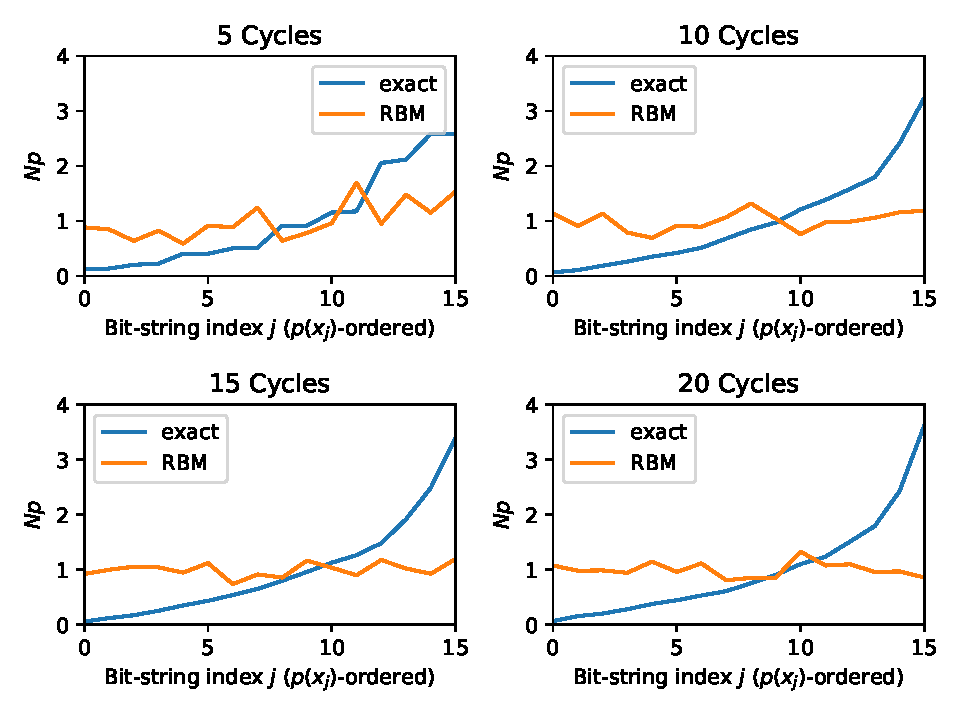
\includegraphics[width=\textwidth]{figures/results/SR-restarts-learned/avgPDF.pdf}
  \caption[Average output probabilities of Stochastic Reconfiguration with Restarts Learned]{
    Average output probabilities of Stochastic Reconfiguration with Restarts Learned. The true 
    output distribution approaches a Porter-Thomas shape with increasing number of cycles.}
  \label{fig:sr_tvd}
\end{figure}

\begin{figure}[H]
  \centering
  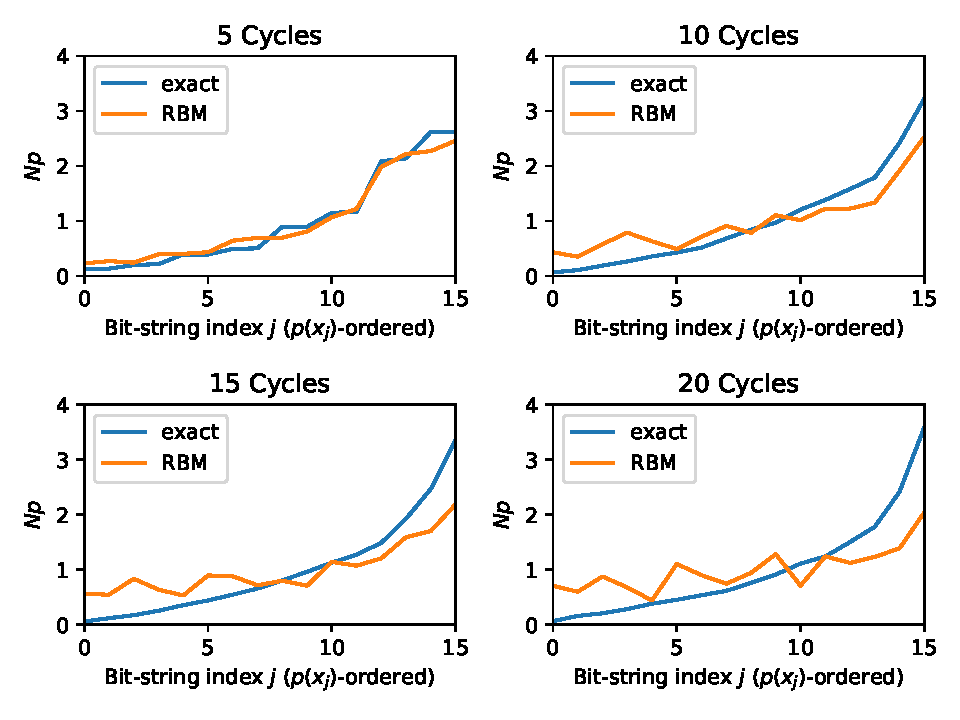
\includegraphics[width=\textwidth]{figures/results/SR-restarts-learned/avgBestPDF.pdf}
  \caption[Averaged best performing output probabilities of Stochastic Reconfiguration with Restarts Learned]{
    Average output probabilities of Stochastic Reconfiguration with Restarts Learned, only RBMs with lowest
    TVD for each circuit are considered. The true 
    output distribution approaches a Porter-Thomas shape with increasing number of cycles.}
  \label{fig:sr_tvd}
\end{figure}

\begin{figure}[H]
  \centering
  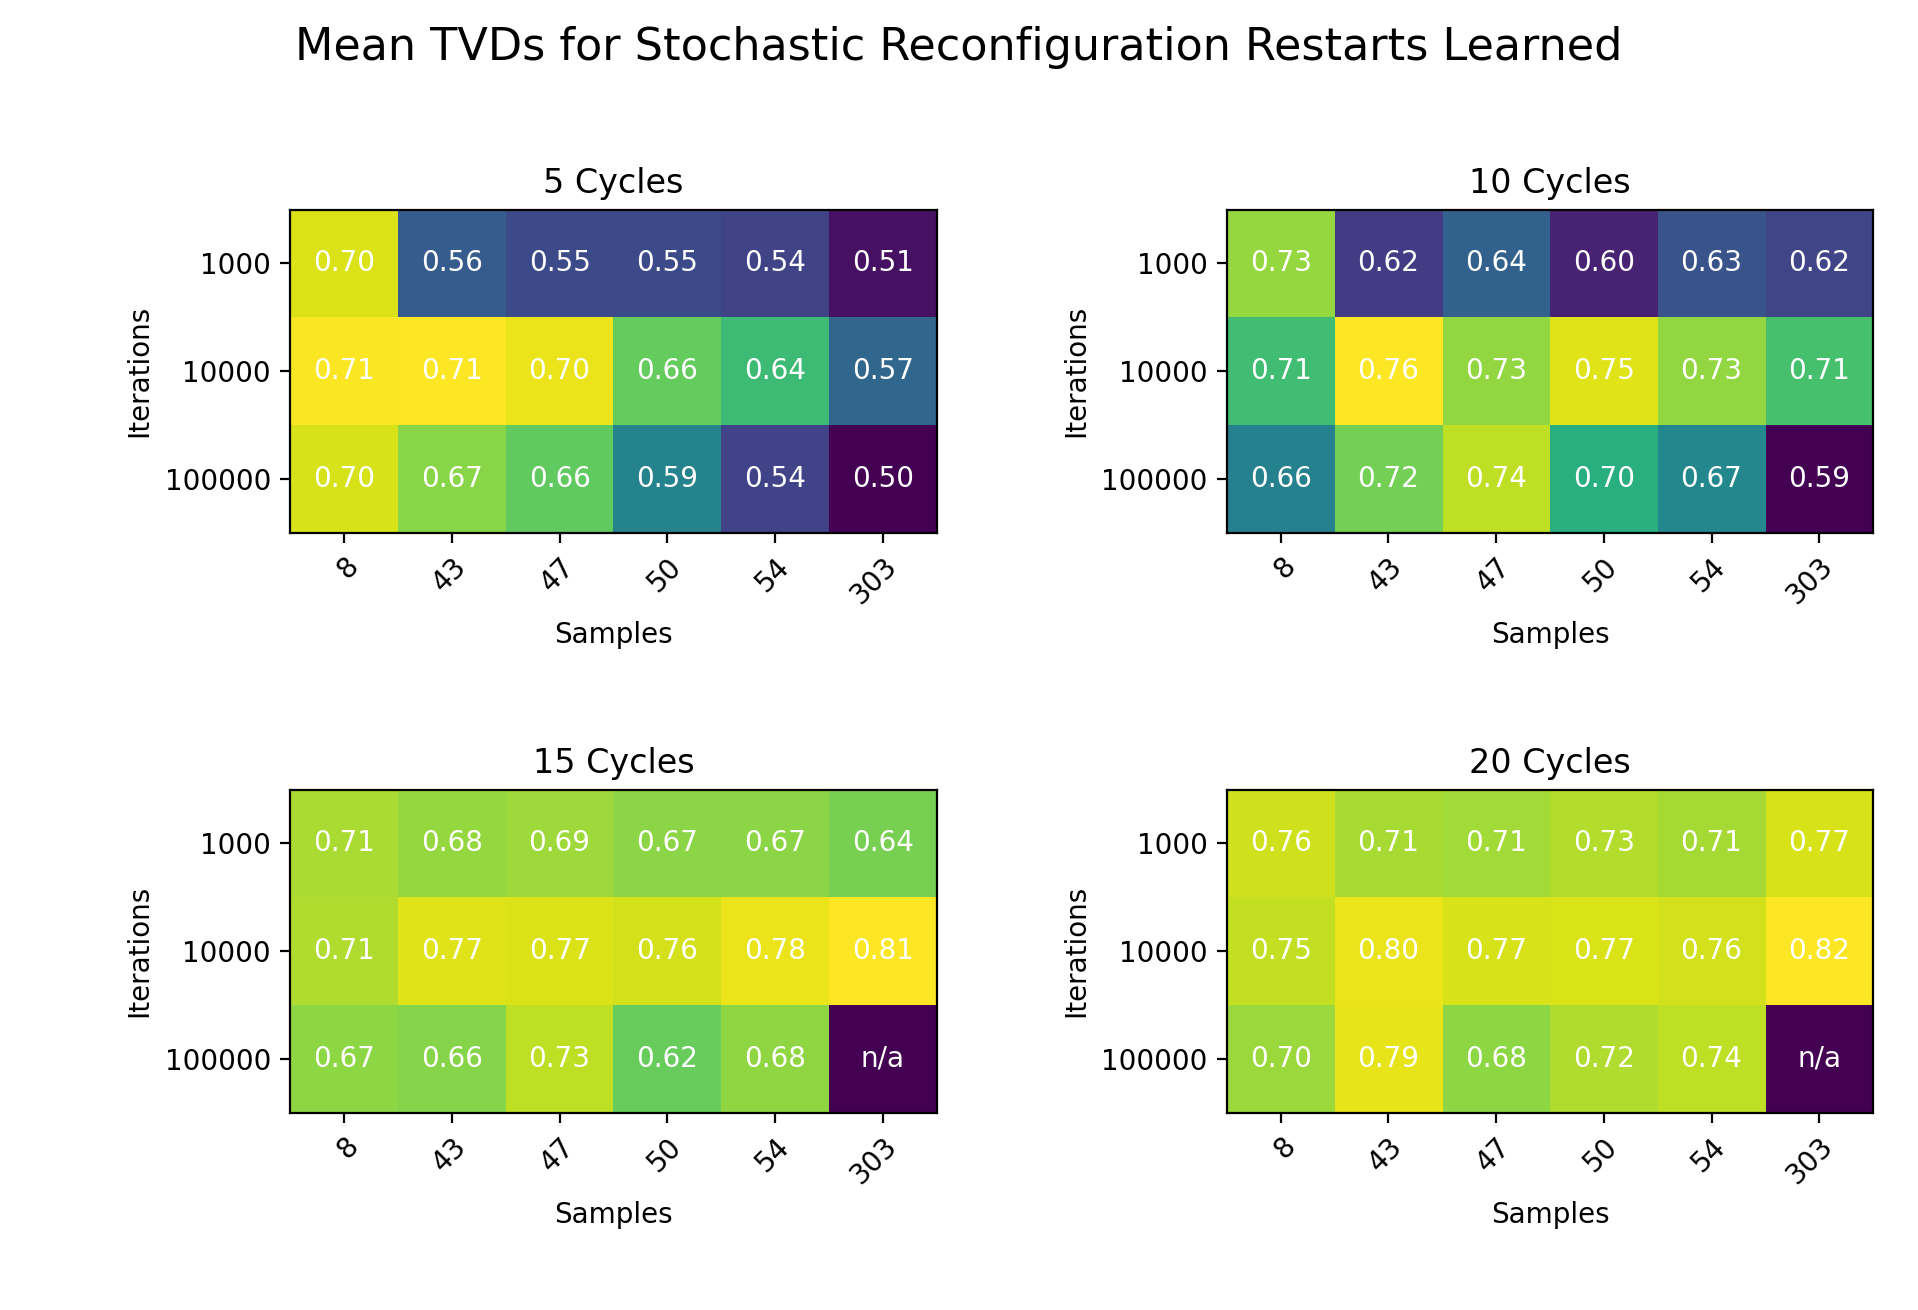
\includegraphics[width=\textwidth]{figures/results/SR-restarts-learned/tvd_heatmap.png}
  \caption[TVD of Stochastic Reconfiguration with Restarts Learned]{TVD of Stochastic 
  Reconfiguration with Restarts Learned for the combinations of iterations and samples tested.
  For 100.000 iterations and 303 samples, the experiments did not finish within the time limit.}
  \label{fig:sr_tvd}
\end{figure}

\begin{figure}[H]
  \centering
  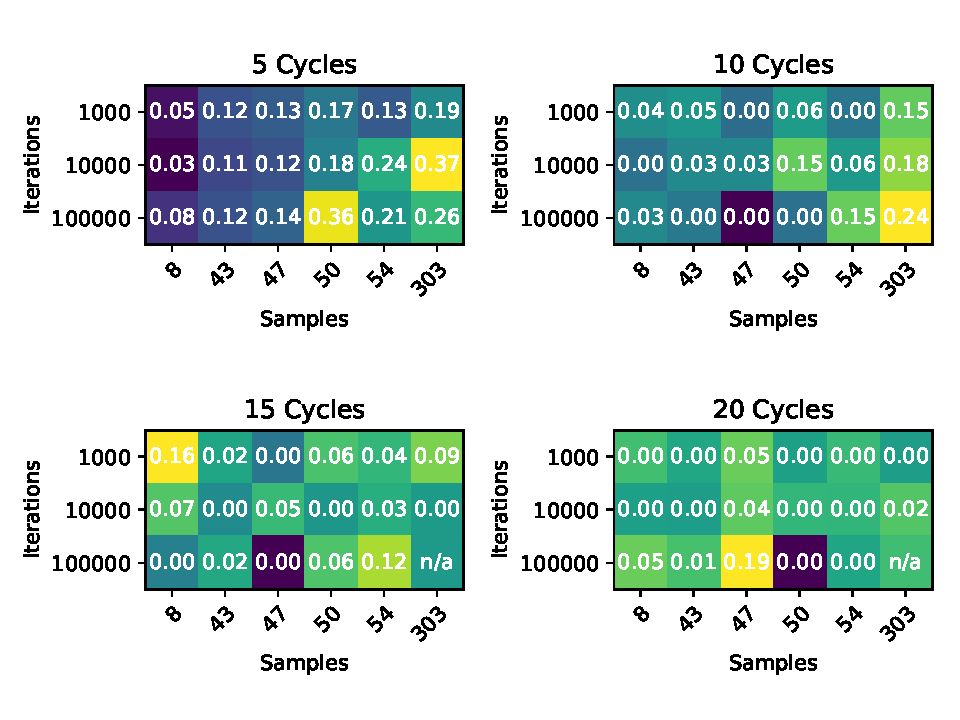
\includegraphics[width=\textwidth]{figures/results/SR-restarts-learned/fxeb_heatmap.pdf}
  \caption[Cross-entropy Fidelity of Stochastic Reconfiguration with Restarts Learned]{Cross-entropy Fidelity of Stochastic 
  Reconfiguration with Restarts Learned for the combinations of iterations and samples tested.
  For 100.000 iterations and 303 samples, the experiments did not finish within the time limit.}
  \label{fig:sr_tvd}
\end{figure}


\begin{figure}[H]
  \centering
  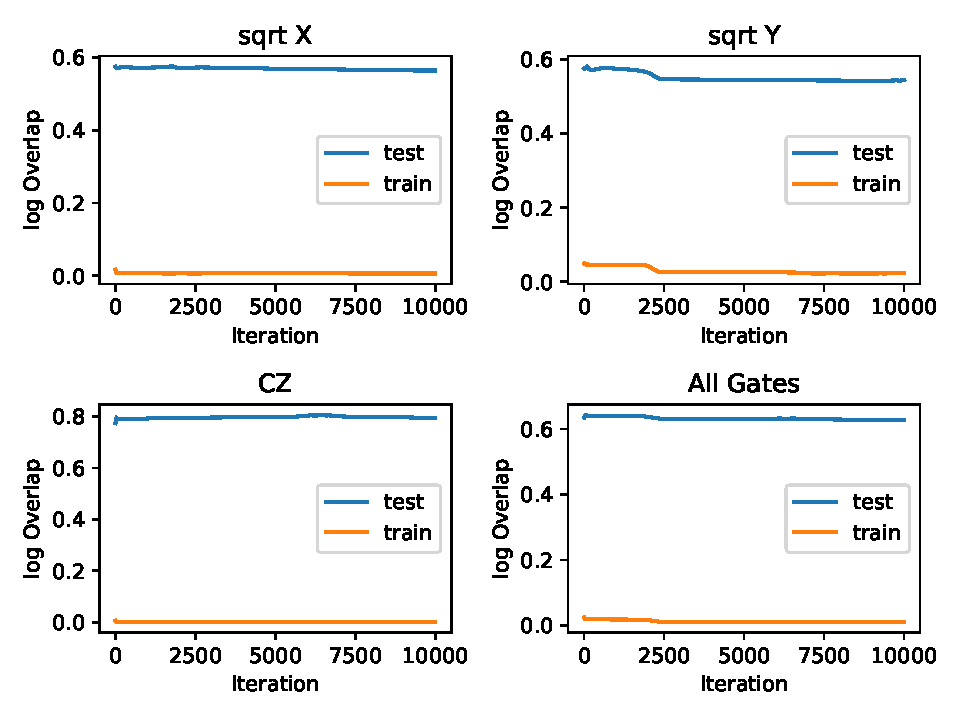
\includegraphics[width=\textwidth]{figures/results/SR-restarts-learned/avgOverlap_8.pdf}
  \caption[Training Overlap of Stochastic Reconfiguration with Restarts Learned]{Training 
  Overlap of Stochastic Reconfiguration with Restarts Learned for 8 samples.}
  \label{fig:sr_tvd}
\end{figure}

\begin{figure}[H]
  \centering
  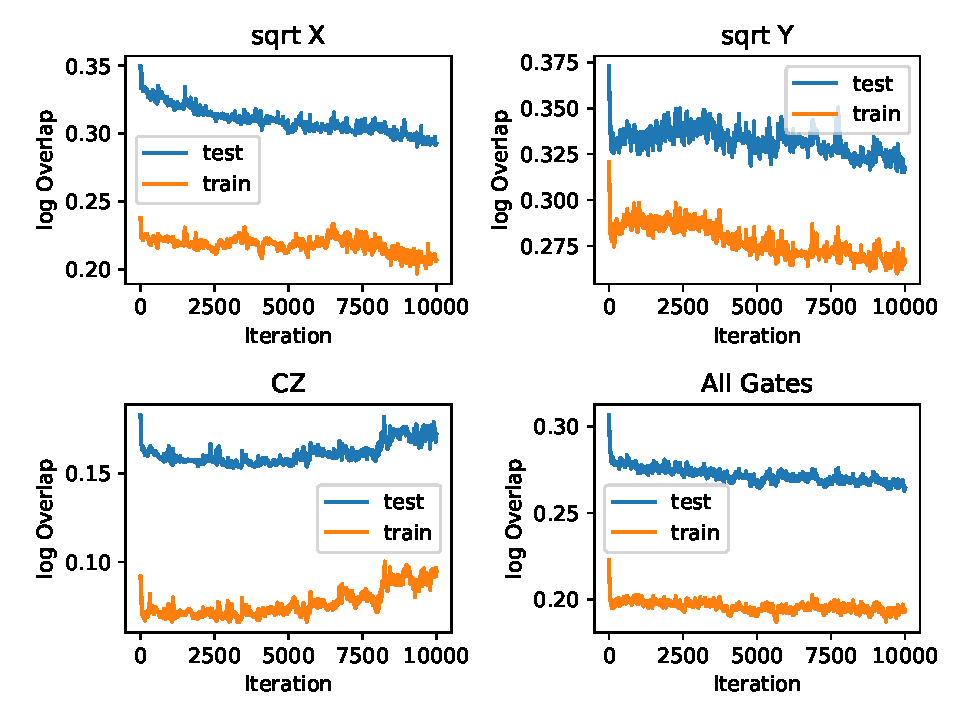
\includegraphics[width=\textwidth]{figures/results/SR-restarts-learned/avgOverlap_47.pdf}
  \caption[Training Overlap of Stochastic Reconfiguration with Restarts Learned]{Training 
  Overlap of Stochastic Reconfiguration with Restarts Learned for 47 samples.}
  \label{fig:sr_tvd}
\end{figure}

\begin{figure}[H]
  \centering
  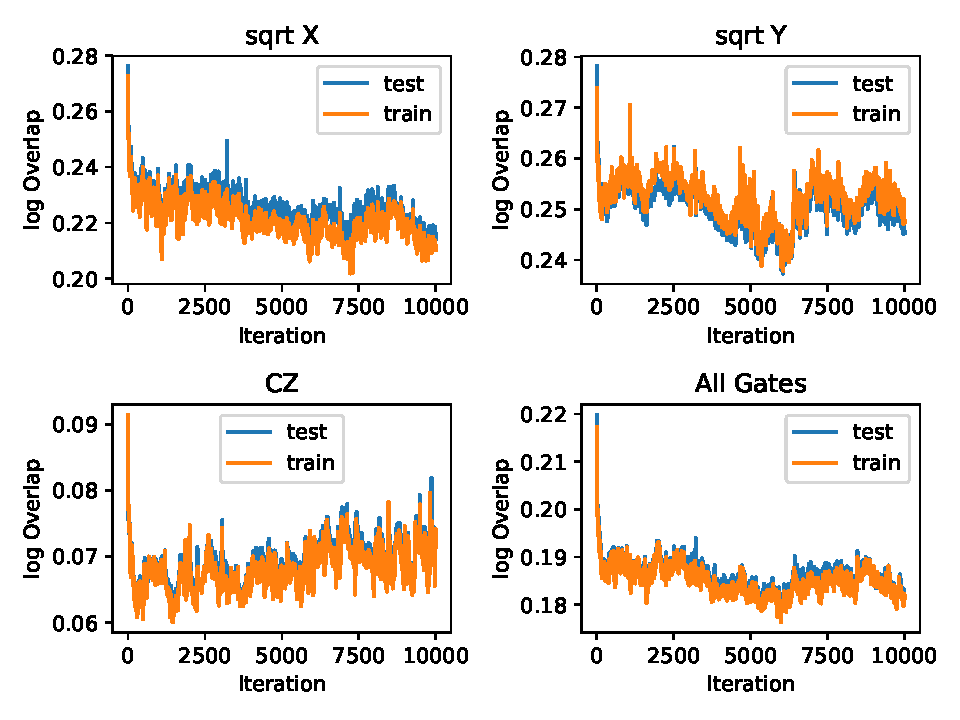
\includegraphics[width=\textwidth]{figures/results/SR-restarts-learned/avgOverlap_303.pdf}
  \caption[Training Overlap of Stochastic Reconfiguration with Restarts Learned]{Training 
  Overlap of Stochastic Reconfiguration with Restarts Learned for 303 samples.}
  \label{fig:sr_tvd}
\end{figure}

\iffalse 
Both Stochastic Reconfiguration and Adamax have been successfully applied to the 
optimization of the parameters of RBMs to classically simulate quantum circuits before \cite{}.
A first direct comparison of these methods for the simulation of random circuits is 
performed in this study. 

Both methods have been used with random restarts and also 
been applied to optimize the parameters of the RBM to simulate $CZ$ gates. 
The TVD of the output of the RBM and the true outputs of the circuits is summarized in 
figure ~\ref{fig:sr_am} for 5, 10, 15 and 20 cycles each.

For 5 cycles, RBMs trained with SR reach an average TVD of $0.61$ with a standard deviation $\sigma$ of 
$\sigma=0.21$. For AdaMax, the average TVD is at $0.48$ with a deviation of $\sigma=0.22$. For 10 cycles, the average TVD is $0.68$ for SR and $0.50$ for AdaMax with standard deviations of 
$\sigma=0.17$ and $0.19$. On 15 cycles, SR reaches a TVD of $0.71$ with a standard deviation of $\sigma=0.16$ and 
AdaMax an average TVD of $0.55$ with $\sigma=0.17$. On the biggest circuits with 20 cycles, RBMs trained with 
SR reach an average TVD of $0.75$ with $\sigma=0.15$ while RBMs optimized with AdaMax reach an 
average TVD of $0.56$ with $\sigma=0.17$. 

\begin{figure}[H]
  \centering
  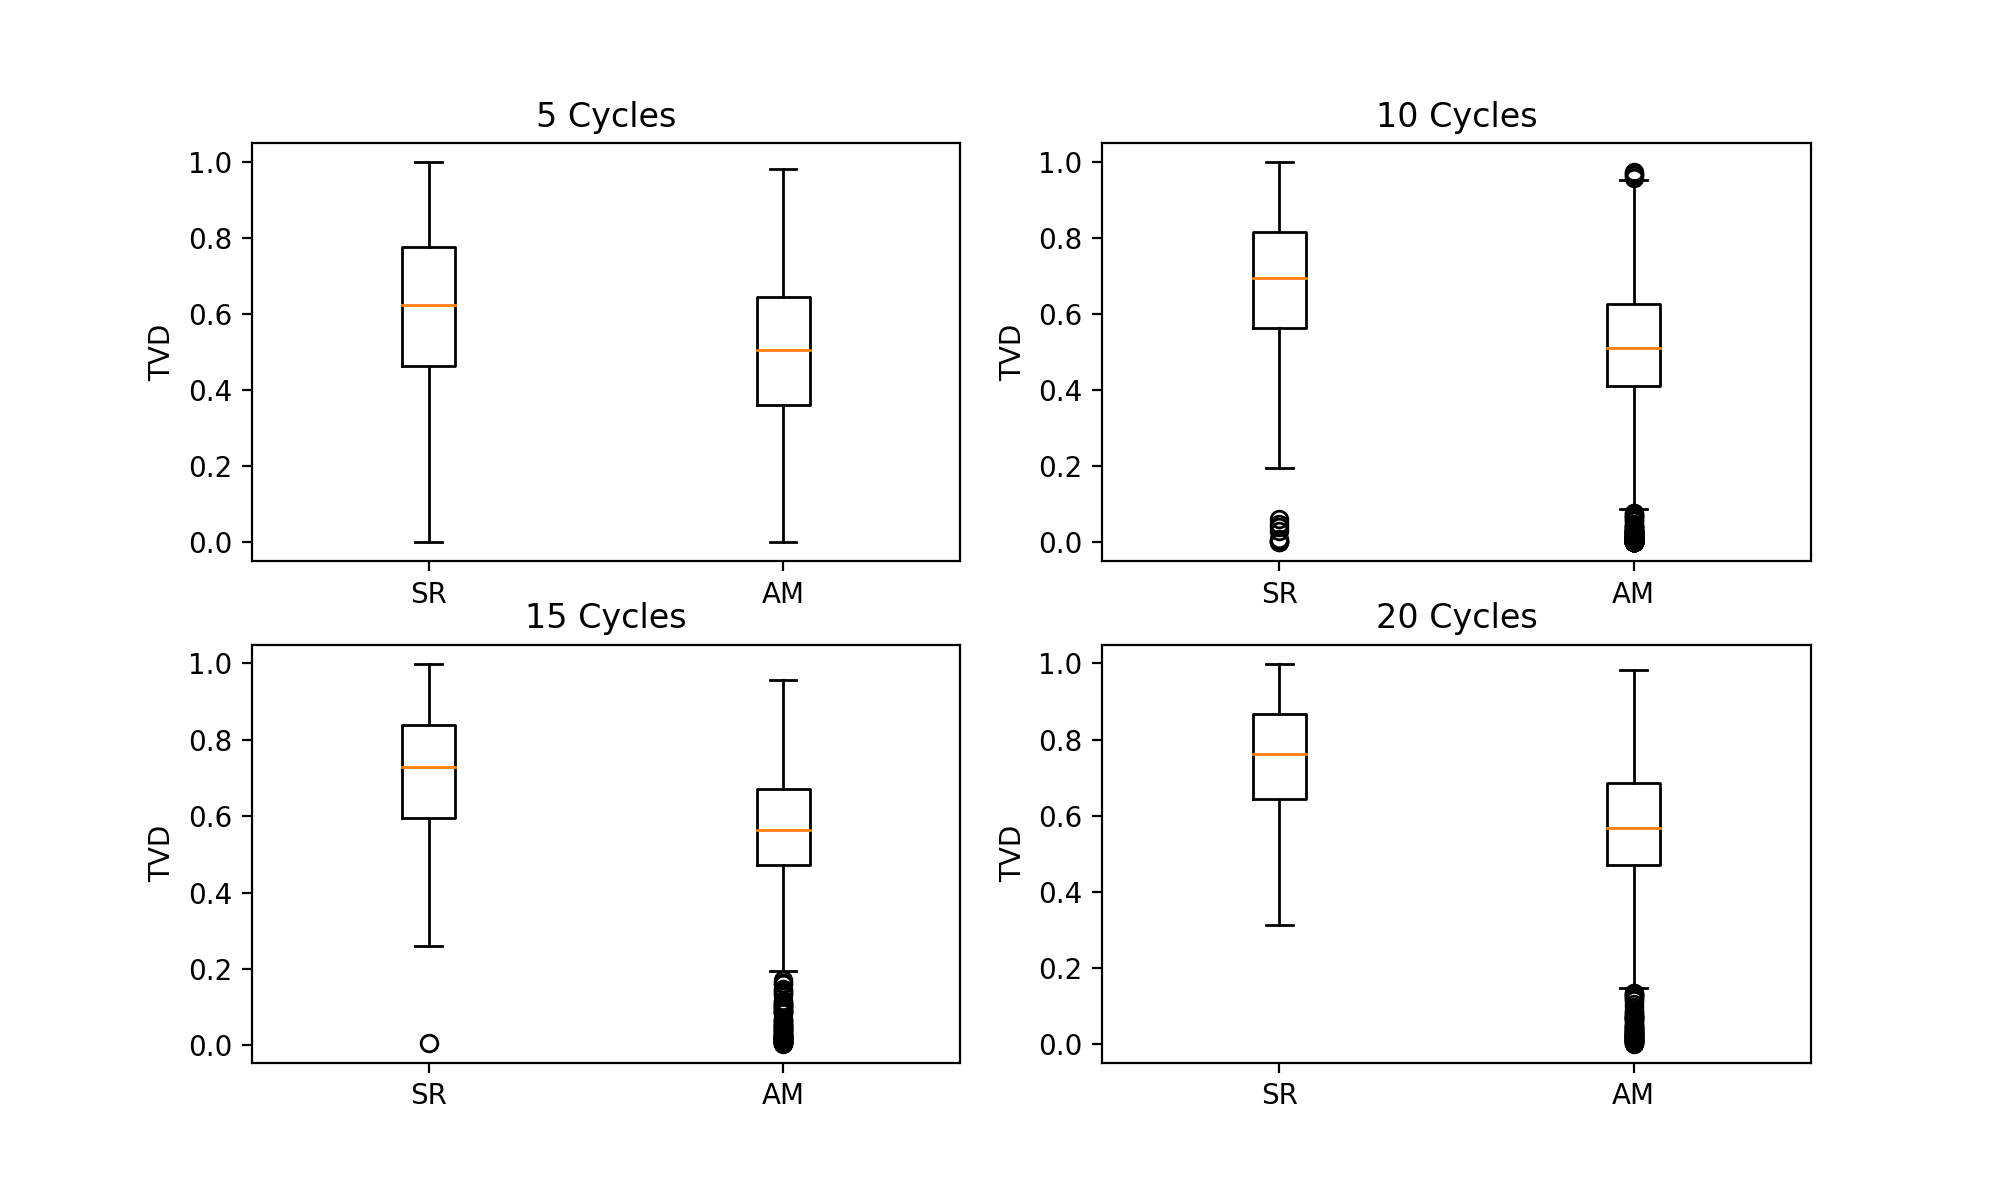
\includegraphics[width=\textwidth]{figures/sr_vs_am.png}
  \caption[Comparison of Stochastic Reconfiguration and AdaMax]{TVD of RBMs trained with 
  Stochastic Reconfiguration (SR) and AdaMax (AM) on random circuits of different depths. Both methods are used with random restarts and also 
  used to optimize the application of $CZ$ gates. TVDs averaged over all number of training samples 
  and iterations.}
  \label{fig:sr_am}
\end{figure}

The $p$ value of the Kruskal-Wallis H test on all circuit instances is $p=0$, suggesting that 
the output distributions of the resulting RBMs trained with both methods differ significantly from
each other. Across all circuit sizes, TVDs with AdaMax have been $24\%$ lower than with SR. 

Some RBMs trained with either method reached TVDs of zero on circuits with a depth of 5, 10, and 15 cycles.
For 20 cycles, however, only AdaMax could optimize some RBMs with a TVD of 0. Also for 10 and 15 cycles, 
the number of RBMs with a TVD of 0 or a value close to 0 is higher for AdaMax than for SR.

The influence of the number of training samples and training iterations on both methods is analyzed in 
sections X to X.
\fi
\subsection{Stochastic Reconfiguration without Random Restarts and CZ Gates Learned}

\begin{figure}[H]
  \centering
  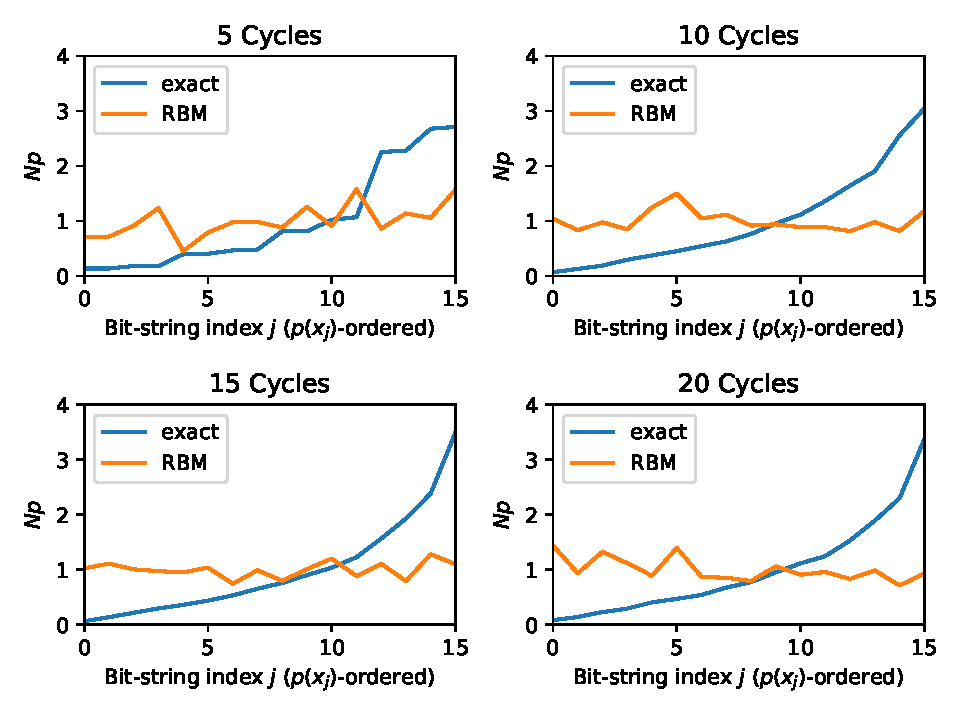
\includegraphics[width=\textwidth]{figures/results/SR-no-restarts-learned/avgPDF.pdf}
  \caption[Average output probabilities of Stochastic Reconfiguration without Restarts Learned]{
    Average output probabilities of Stochastic Reconfiguration without Restarts Learned. The true 
    output distribution approaches a Porter-Thomas shape with increasing number of cycles.}
  \label{fig:sr_tvd}
\end{figure}

\begin{figure}[H]
  \centering
  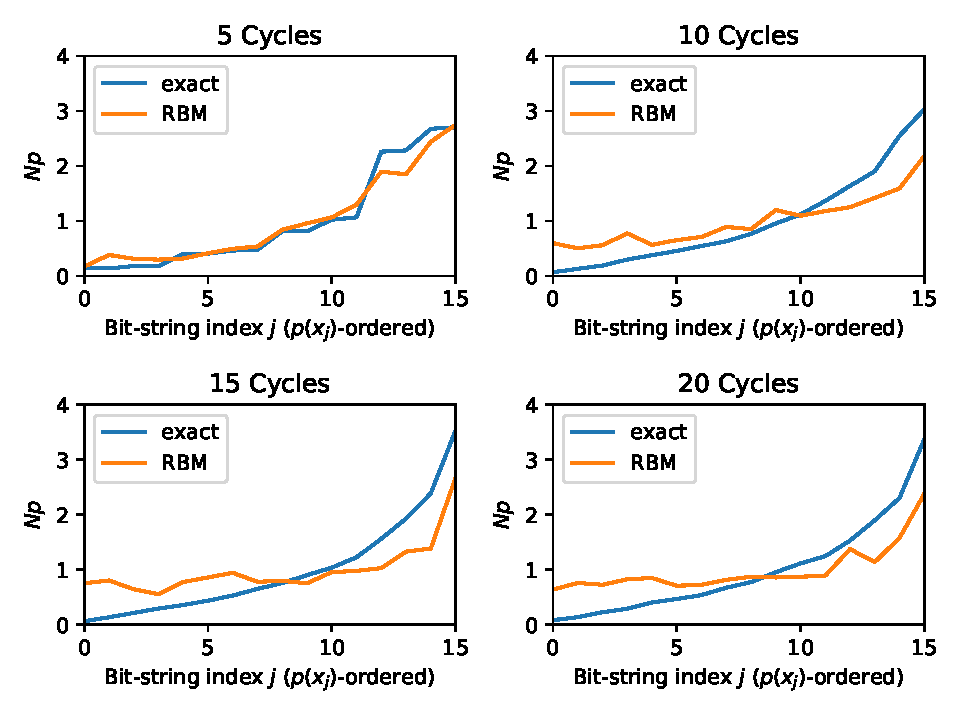
\includegraphics[width=\textwidth]{figures/results/SR-no-restarts-learned/avgBestPDF.pdf}
  \caption[Averaged best performing output probabilities of Stochastic Reconfiguration without Restarts Learned]{
    Average output probabilities of Stochastic Reconfiguration without Restarts Learned, only RBMs with lowest
    TVD for each circuit are considered. The true 
    output distribution approaches a Porter-Thomas shape with increasing number of cycles.}
  \label{fig:sr_tvd}
\end{figure}

\begin{figure}[H]
  \centering
  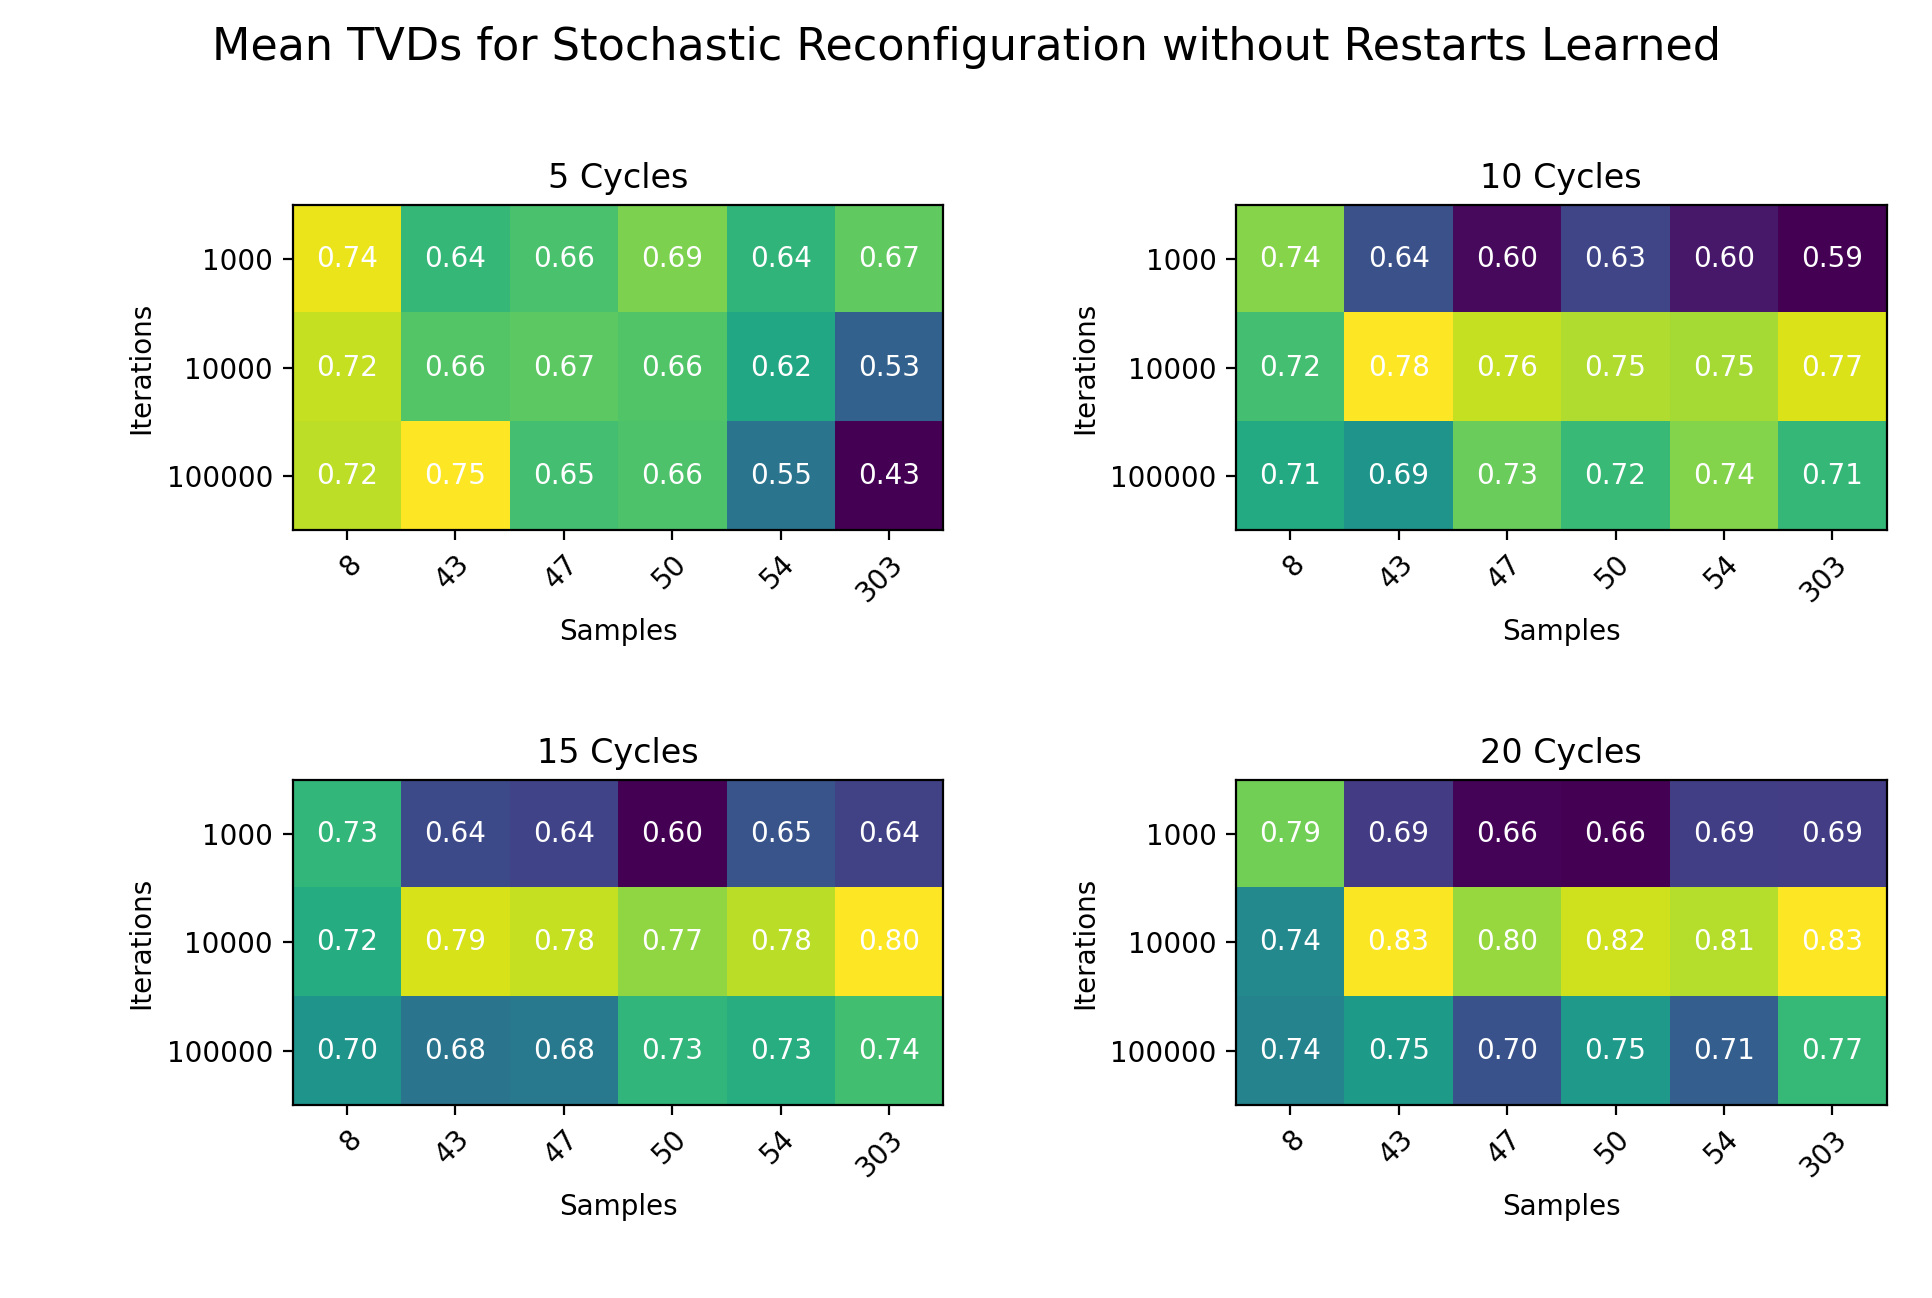
\includegraphics[width=\textwidth]{figures/results/SR-no-restarts-learned/tvd_heatmap.png}
  \caption[TVD of Stochastic Reconfiguration without Restarts Learned]{TVD of Stochastic 
  Reconfiguration without Restarts Learned for the combinations of iterations and samples tested.
  For 100.000 iterations and 303 samples, the experiments did not finish within the time limit.}
  \label{fig:sr_tvd}
\end{figure}

\begin{figure}[H]
  \centering
  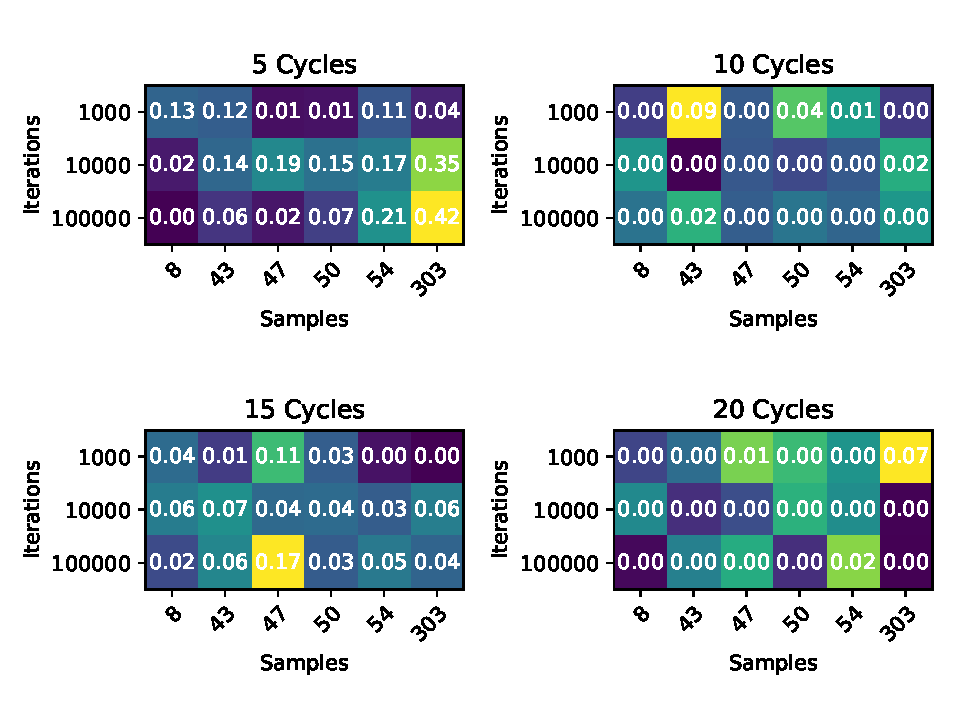
\includegraphics[width=\textwidth]{figures/results/SR-no-restarts-learned/fxeb_heatmap.pdf}
  \caption[Cross-entropy Fidelity of Stochastic Reconfiguration without Restarts Learned]{Cross-entropy Fidelity of Stochastic 
  Reconfiguration without Restarts Learned for the combinations of iterations and samples tested.
  For 100.000 iterations and 303 samples, the experiments did not finish within the time limit.}
  \label{fig:sr_tvd}
\end{figure}


\begin{figure}[H]
  \centering
  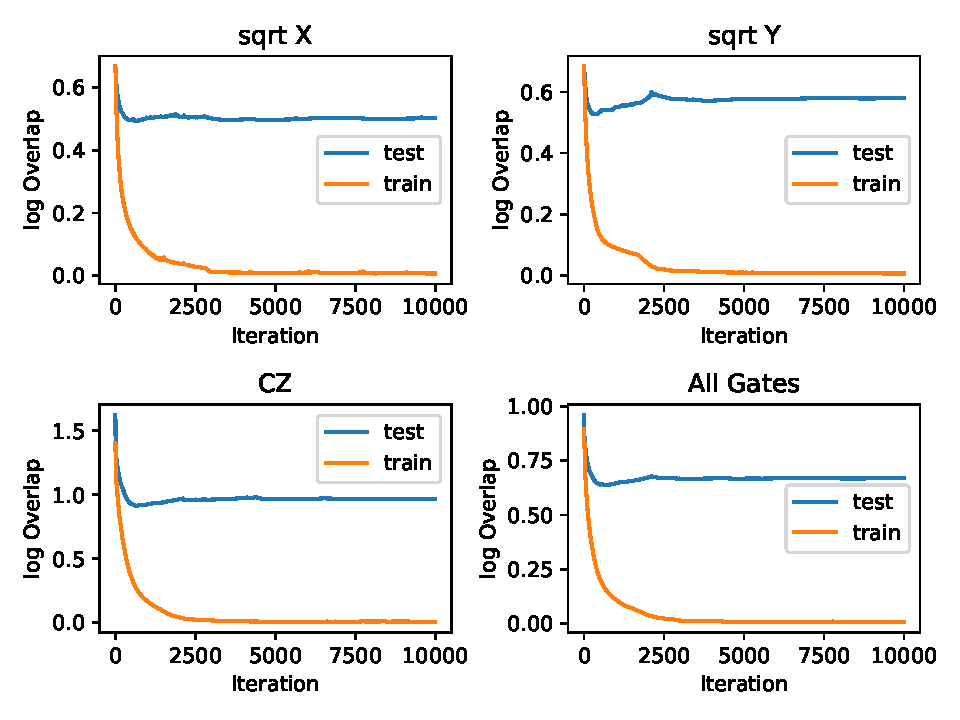
\includegraphics[width=\textwidth]{figures/results/SR-no-restarts-learned/avgOverlap_8.pdf}
  \caption[Training Overlap of Stochastic Reconfiguration without Restarts Learned]{Training 
  Overlap of Stochastic Reconfiguration without Restarts Learned for 8 samples.}
  \label{fig:sr_tvd}
\end{figure}

\begin{figure}[H]
  \centering
  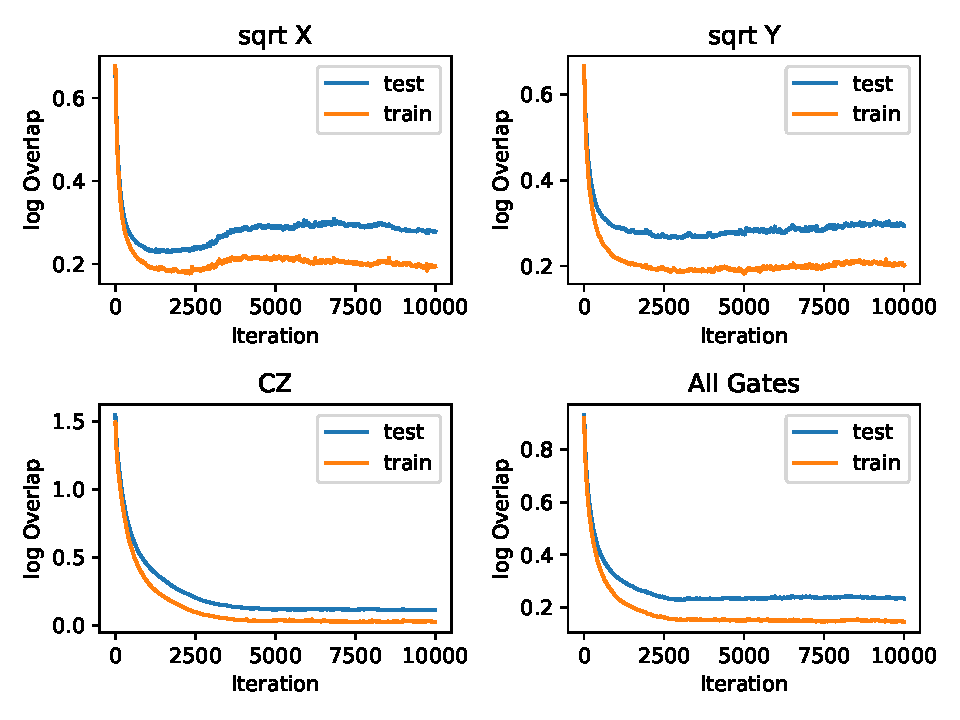
\includegraphics[width=\textwidth]{figures/results/SR-no-restarts-learned/avgOverlap_47.pdf}
  \caption[Training Overlap of Stochastic Reconfiguration without Restarts Learned]{Training 
  Overlap of Stochastic Reconfiguration without Restarts Learned for 47 samples.}
  \label{fig:sr_tvd}
\end{figure}

\begin{figure}[H]
  \centering
  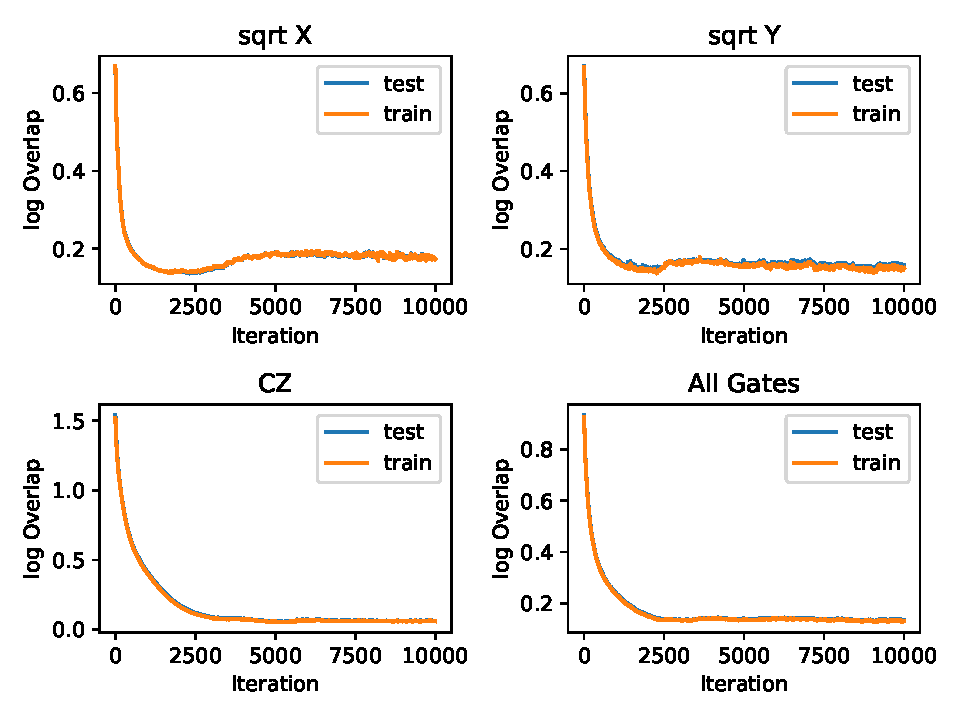
\includegraphics[width=\textwidth]{figures/results/SR-no-restarts-learned/avgOverlap_303.pdf}
  \caption[Training Overlap of Stochastic Reconfiguration without Restarts Learned]{Training 
  Overlap of Stochastic Reconfiguration without Restarts Learned for 303 samples.}
  \label{fig:sr_tvd}
\end{figure}

\iffalse
Introducing random restarts into stochastic optimization algorithms is a common technique to improve 
performance \cite{}. Other works on classical simulation of quantum systems don't mention the use
of random restarts in their studies \cite{}. To our knowledge, this study is the first to directly compare 
the SR method with and without random restarts in the optimization of RBM parameters 
for the simulation of quantum circuits.

Again, both methods have also been used to optimize the parameters of the RBM to simulate $CZ$ gates. 
The TVD of the output of the RBM and the true outputs of the circuits is summarized in 
figure ~\ref{fig:sr_restarts} for 5, 10, 15 and 20 cycles each.

For 5 cycles, RBMs trained without random restarts reach an average TVD of $0.66$ with a standard deviation of
$\sigma=0.21$ ($0.61$ and $0.21$ with restarts). For 10 cycles, the average TVD is $0.69$ and
$\sigma=0.17$ ($0.68$ and $0.17$ with restarts). On 15 cycles, without restarts the TVD is at $0.71$ with a standard deviation of $\sigma=0.16$
(same values as with restarts). On the biggest circuits with 20 cycles, RBMs trained without
restarts reach an average TVD of $0.75$ with $\sigma=0.15$ (same values as with restarts).

\begin{figure}[H]
  \centering
  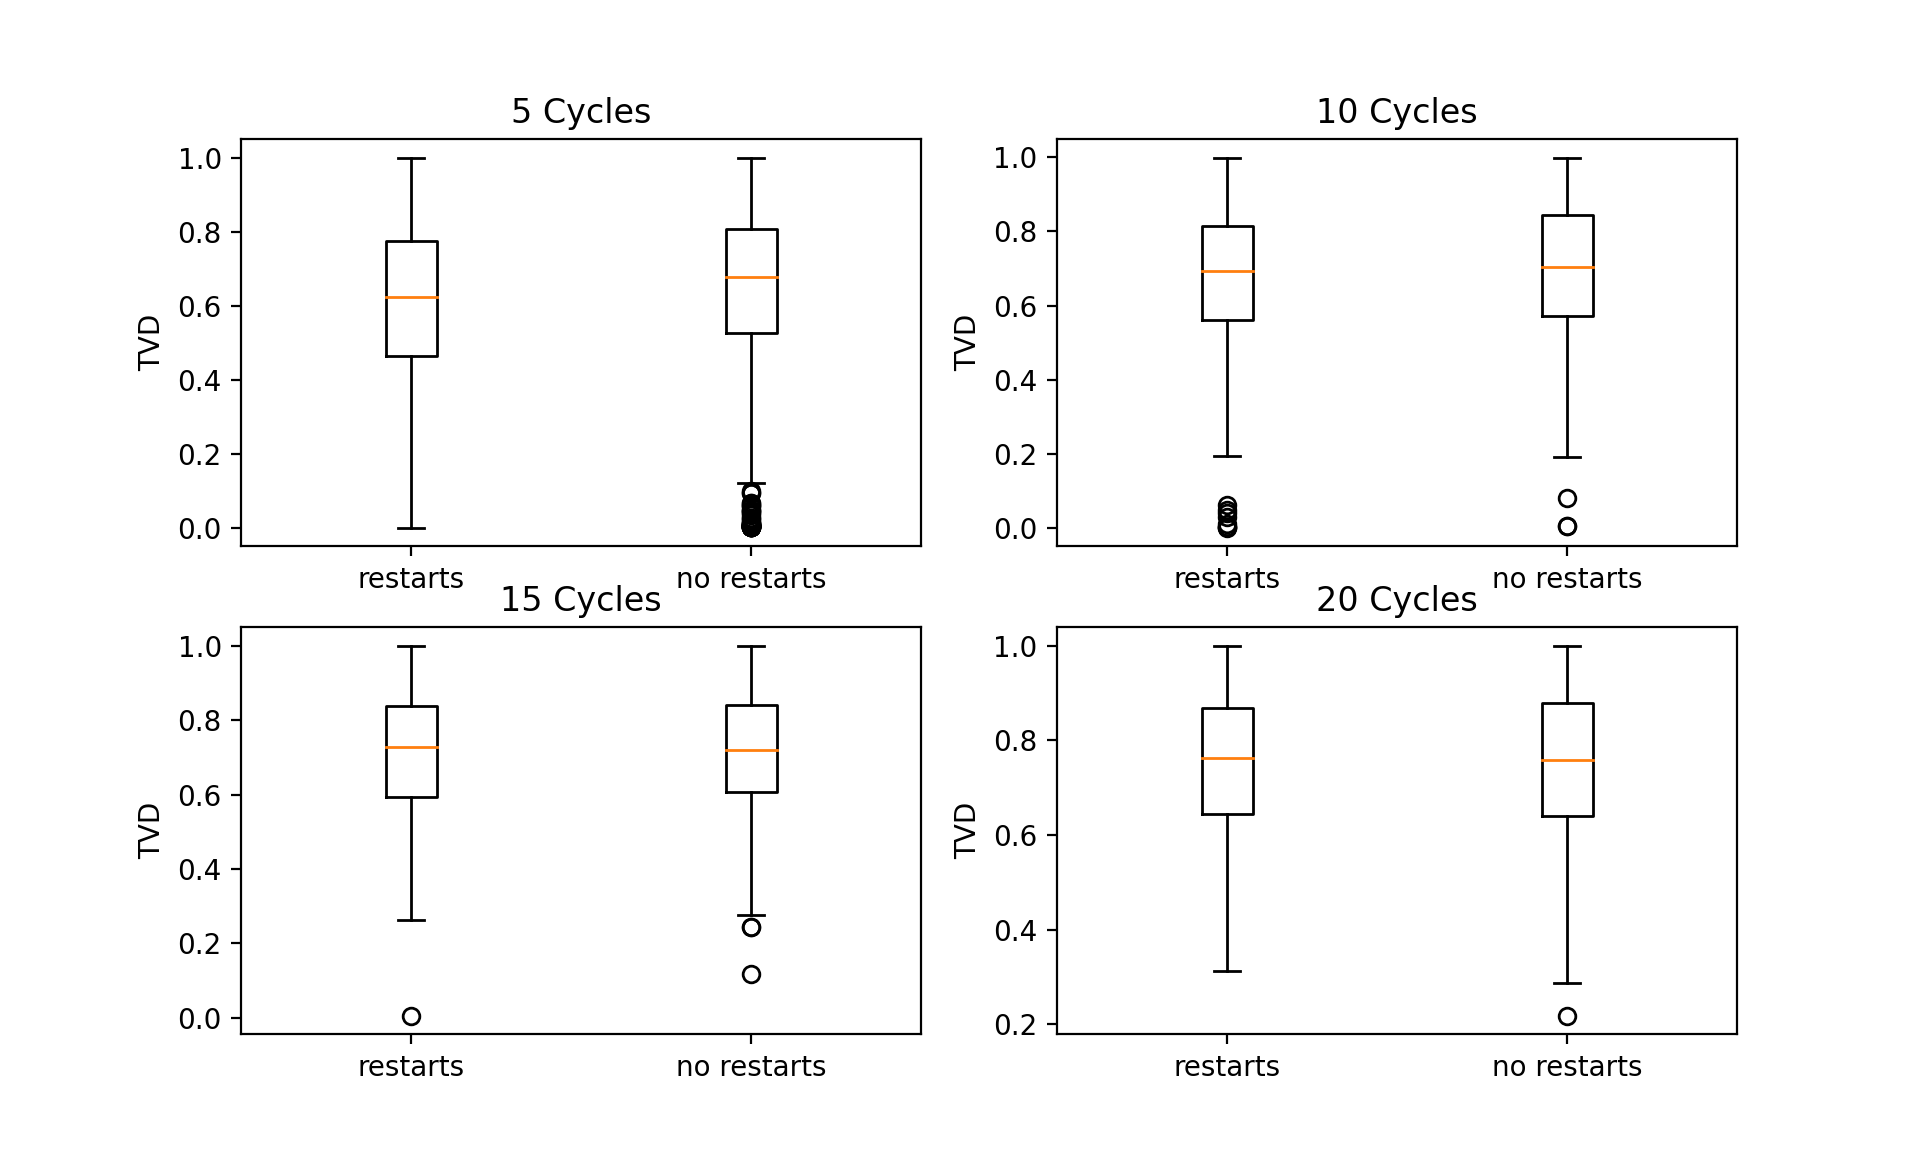
\includegraphics[width=\textwidth]{figures/sr_restarts.png}
  \caption[Comparison of Stochastic Reconfiguration with and without random restarts]{TVD of RBMs trained with 
  Stochastic Reconfiguration with and without random restarts on random circuits of different depths. Both methods are also used  
  used to optimize the application of $CZ$ gates. TVDs averaged over all number of training samples 
  and iterations.}
  \label{fig:sr_restarts}
\end{figure}


The $p$ value of the Kruskal-Wallis H test on all circuit instances is $p=0$ also in this case, suggesting that 
that random restarts have a significant impact on the training process. Across all circuit sizes, TVDs with restarts have been $2\%$ lower than without them. 


The optimal results with both methods are similar. They are analysed in more depth in section X.
The influence of the number of training samples and training iterations on both methods is analyzed in 
sections X and X.
\fi
\subsection{Stochastic Reconfiguration with Random Restarts and CZ Gates Applied Exactly}

\begin{figure}[H]
  \centering
  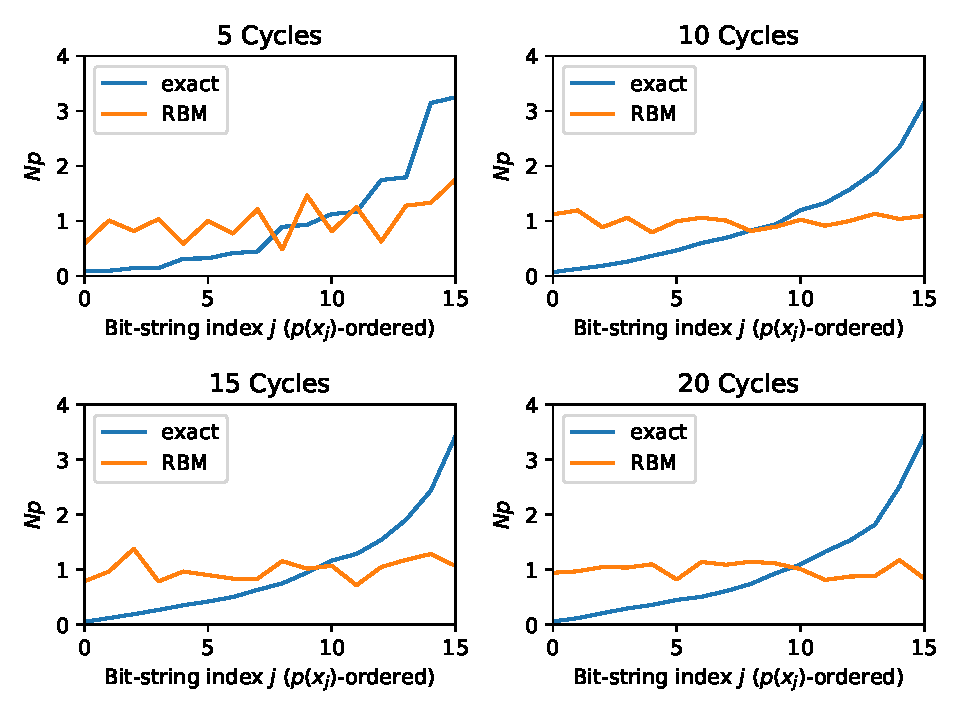
\includegraphics[width=\textwidth]{figures/results/SR-restarts-not-learned/avgPDF.pdf}
  \caption[Average output probabilities of Stochastic Reconfiguration with Restarts Exact]{
    Average output probabilities of Stochastic Reconfiguration with Restarts Exact. The true 
    output distribution approaches a Porter-Thomas shape with increasing number of cycles.}
  \label{fig:sr_tvd}
\end{figure}

\begin{figure}[H]
  \centering
  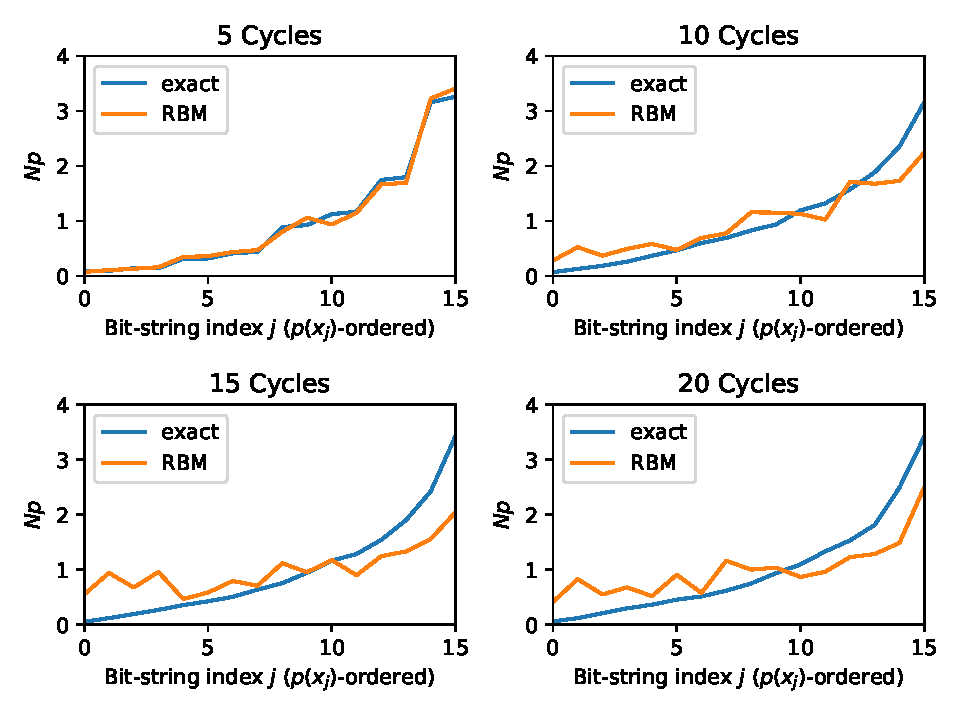
\includegraphics[width=\textwidth]{figures/results/SR-restarts-not-learned/avgBestPDF.pdf}
  \caption[Averaged best performing output probabilities of Stochastic Reconfiguration with Restarts Exact]{
    Average output probabilities of Stochastic Reconfiguration with Restarts Exact, only RBMs with lowest
    TVD for each circuit are considered. The true 
    output distribution approaches a Porter-Thomas shape with increasing number of cycles.}
  \label{fig:sr_tvd}
\end{figure}

\begin{figure}[H]
  \centering
  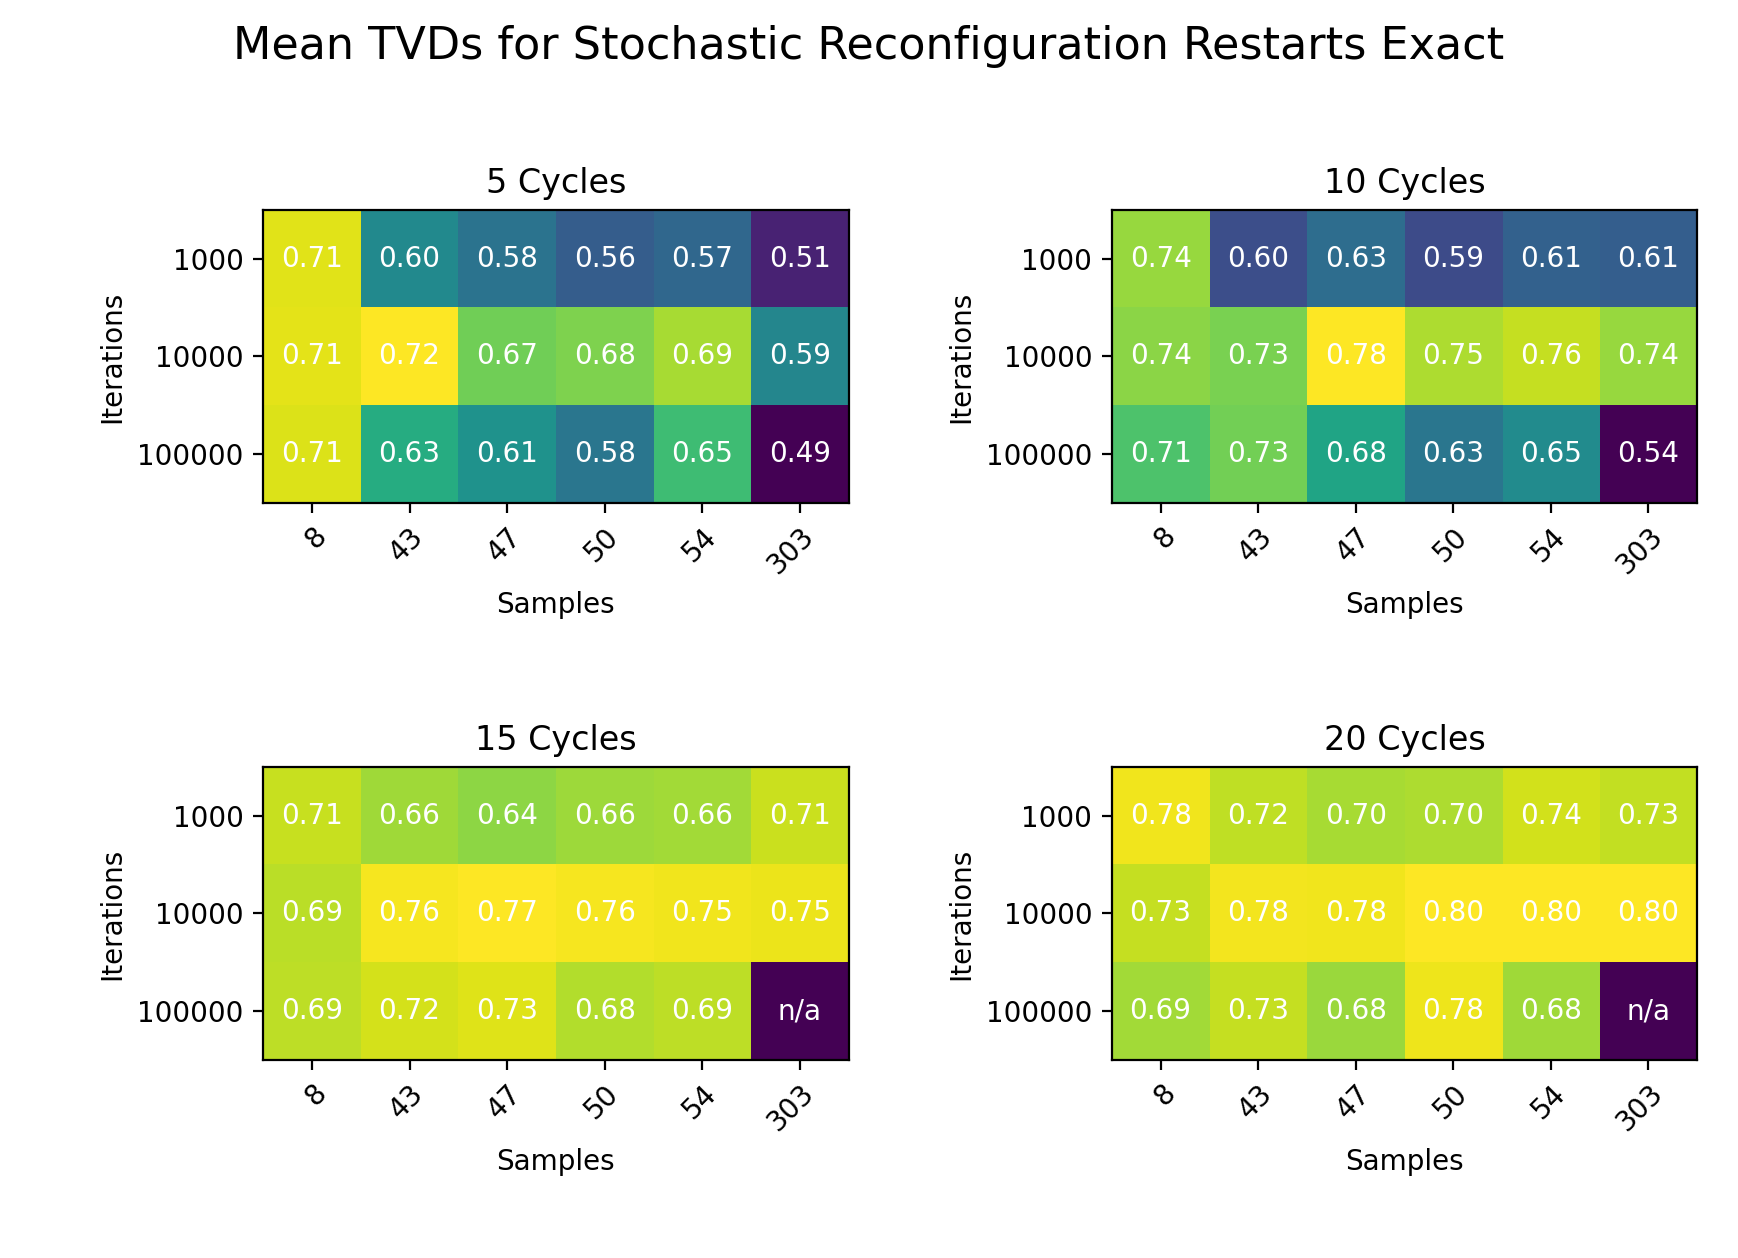
\includegraphics[width=\textwidth]{figures/results/SR-restarts-not-learned/tvd_heatmap.png}
  \caption[TVD of Stochastic Reconfiguration with Restarts Exact]{TVD of Stochastic 
  Reconfiguration with Restarts Exact for the combinations of iterations and samples tested.
  For 100.000 iterations and 303 samples, the experiments did not finish within the time limit.}
  \label{fig:sr_tvd}
\end{figure}

\begin{figure}[H]
  \centering
  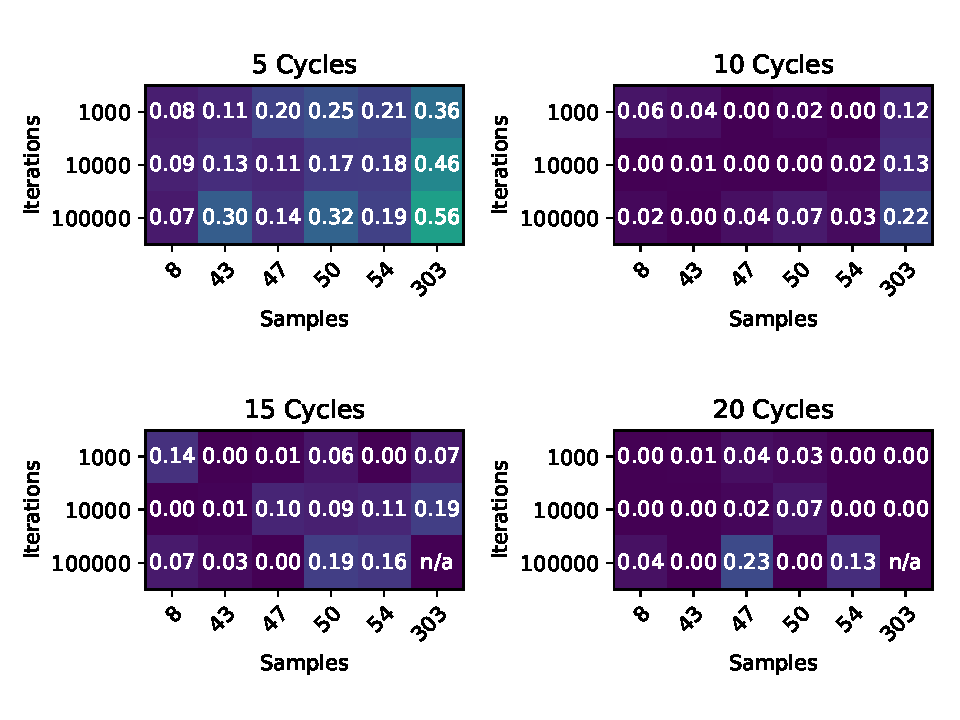
\includegraphics[width=\textwidth]{figures/results/SR-restarts-not-learned/fxeb_heatmap.pdf}
  \caption[Cross-entropy Fidelity of Stochastic Reconfiguration with Restarts Exact]{Cross-entropy Fidelity of Stochastic 
  Reconfiguration with Restarts Exact for the combinations of iterations and samples tested.
  For 100.000 iterations and 303 samples, the experiments did not finish within the time limit.}
  \label{fig:sr_tvd}
\end{figure}


\begin{figure}[H]
  \centering
  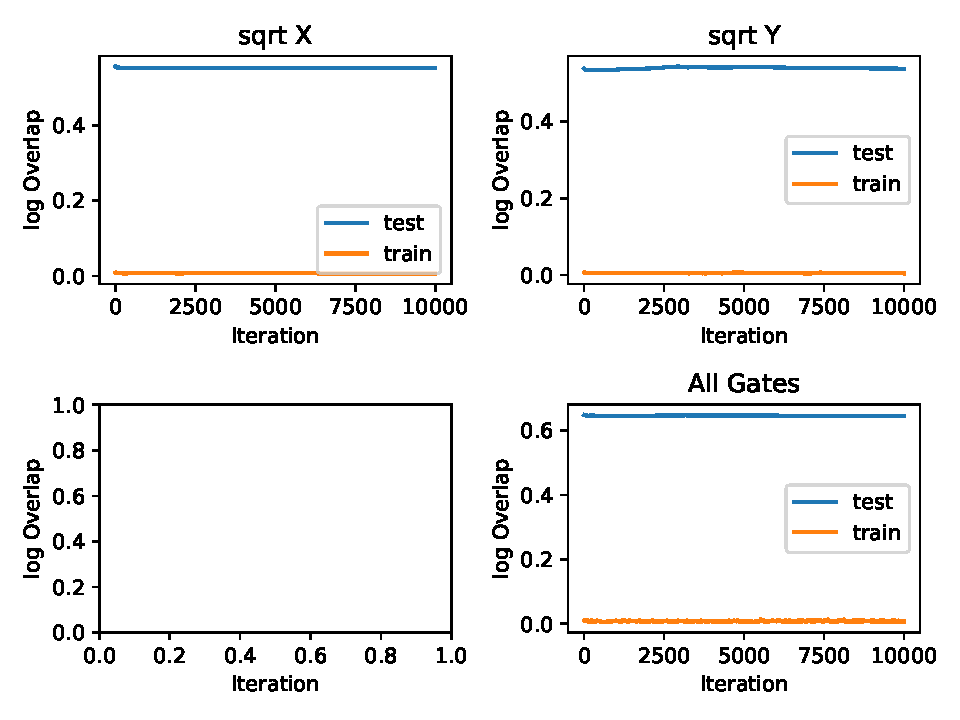
\includegraphics[width=\textwidth]{figures/results/SR-restarts-not-learned/avgOverlap_8.pdf}
  \caption[Training Overlap of Stochastic Reconfiguration with Restarts Exact]{Training 
  Overlap of Stochastic Reconfiguration with Restarts Exact for 8 samples.}
  \label{fig:sr_tvd}
\end{figure}

\begin{figure}[H]
  \centering
  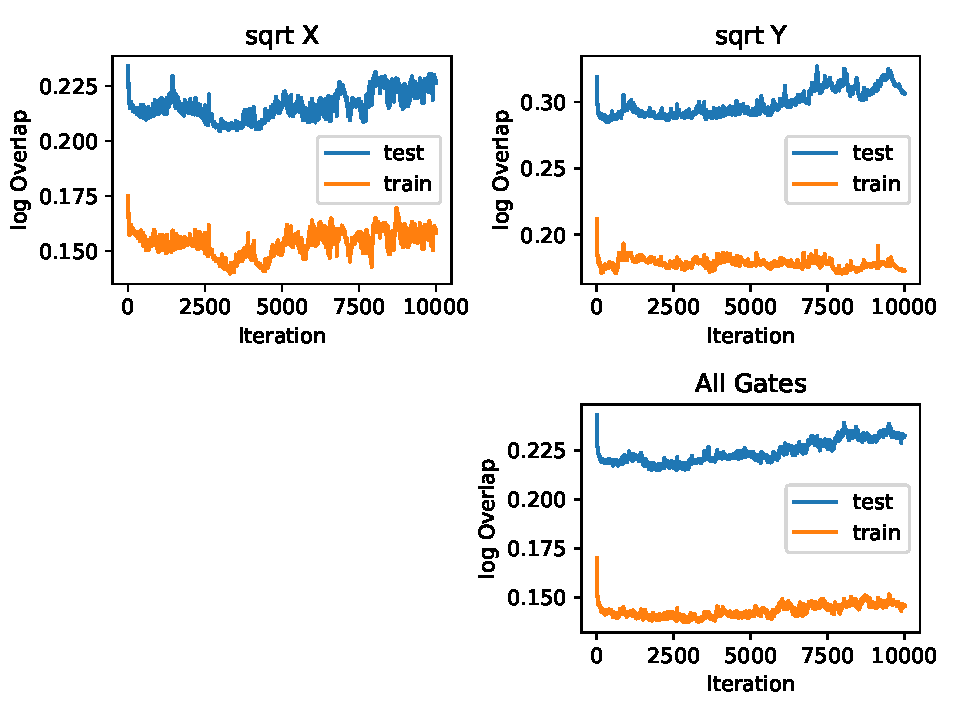
\includegraphics[width=\textwidth]{figures/results/SR-restarts-not-learned/avgOverlap_47.pdf}
  \caption[Training Overlap of Stochastic Reconfiguration with Restarts Exact]{Training 
  Overlap of Stochastic Reconfiguration with Restarts Exact for 47 samples.}
  \label{fig:sr_tvd}
\end{figure}

\begin{figure}[H]
  \centering
  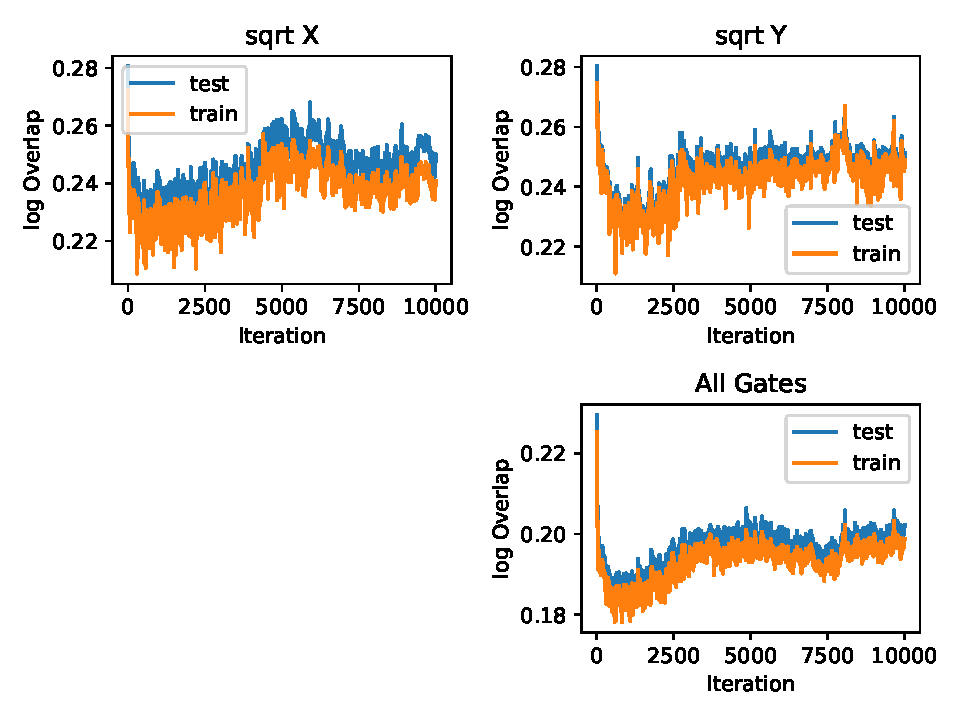
\includegraphics[width=\textwidth]{figures/results/SR-restarts-not-learned/avgOverlap_303.pdf}
  \caption[Training Overlap of Stochastic Reconfiguration with Restarts Exact]{Training 
  Overlap of Stochastic Reconfiguration with Restarts Exact for 303 samples.}
  \label{fig:sr_tvd}
\end{figure}

\iffalse
So far, applying a $CZ$ gate to the quantum state represented by a RBM, has always done 
by adapting the parameters of the RBM directly as described in section X. To understand the 
implications of adding additional hidden units on following training processes on the RBM when 
applying single qubit gates, different experiments have been run to once applying the $CZ$ gate 
exactly with rules and once by using the approach to adapt the parameters in an iterative training 
process.

Both times, the all training phases of the RBM happened with Stochastic Reconfiguration and random restarts.
The TVD of the output of the RBM and the true outputs of the circuits is summarized in 
figure ~\ref{fig:sr_learned} for 5, 10, 15 and 20 cycles each.


\begin{figure}[H]
    \centering
    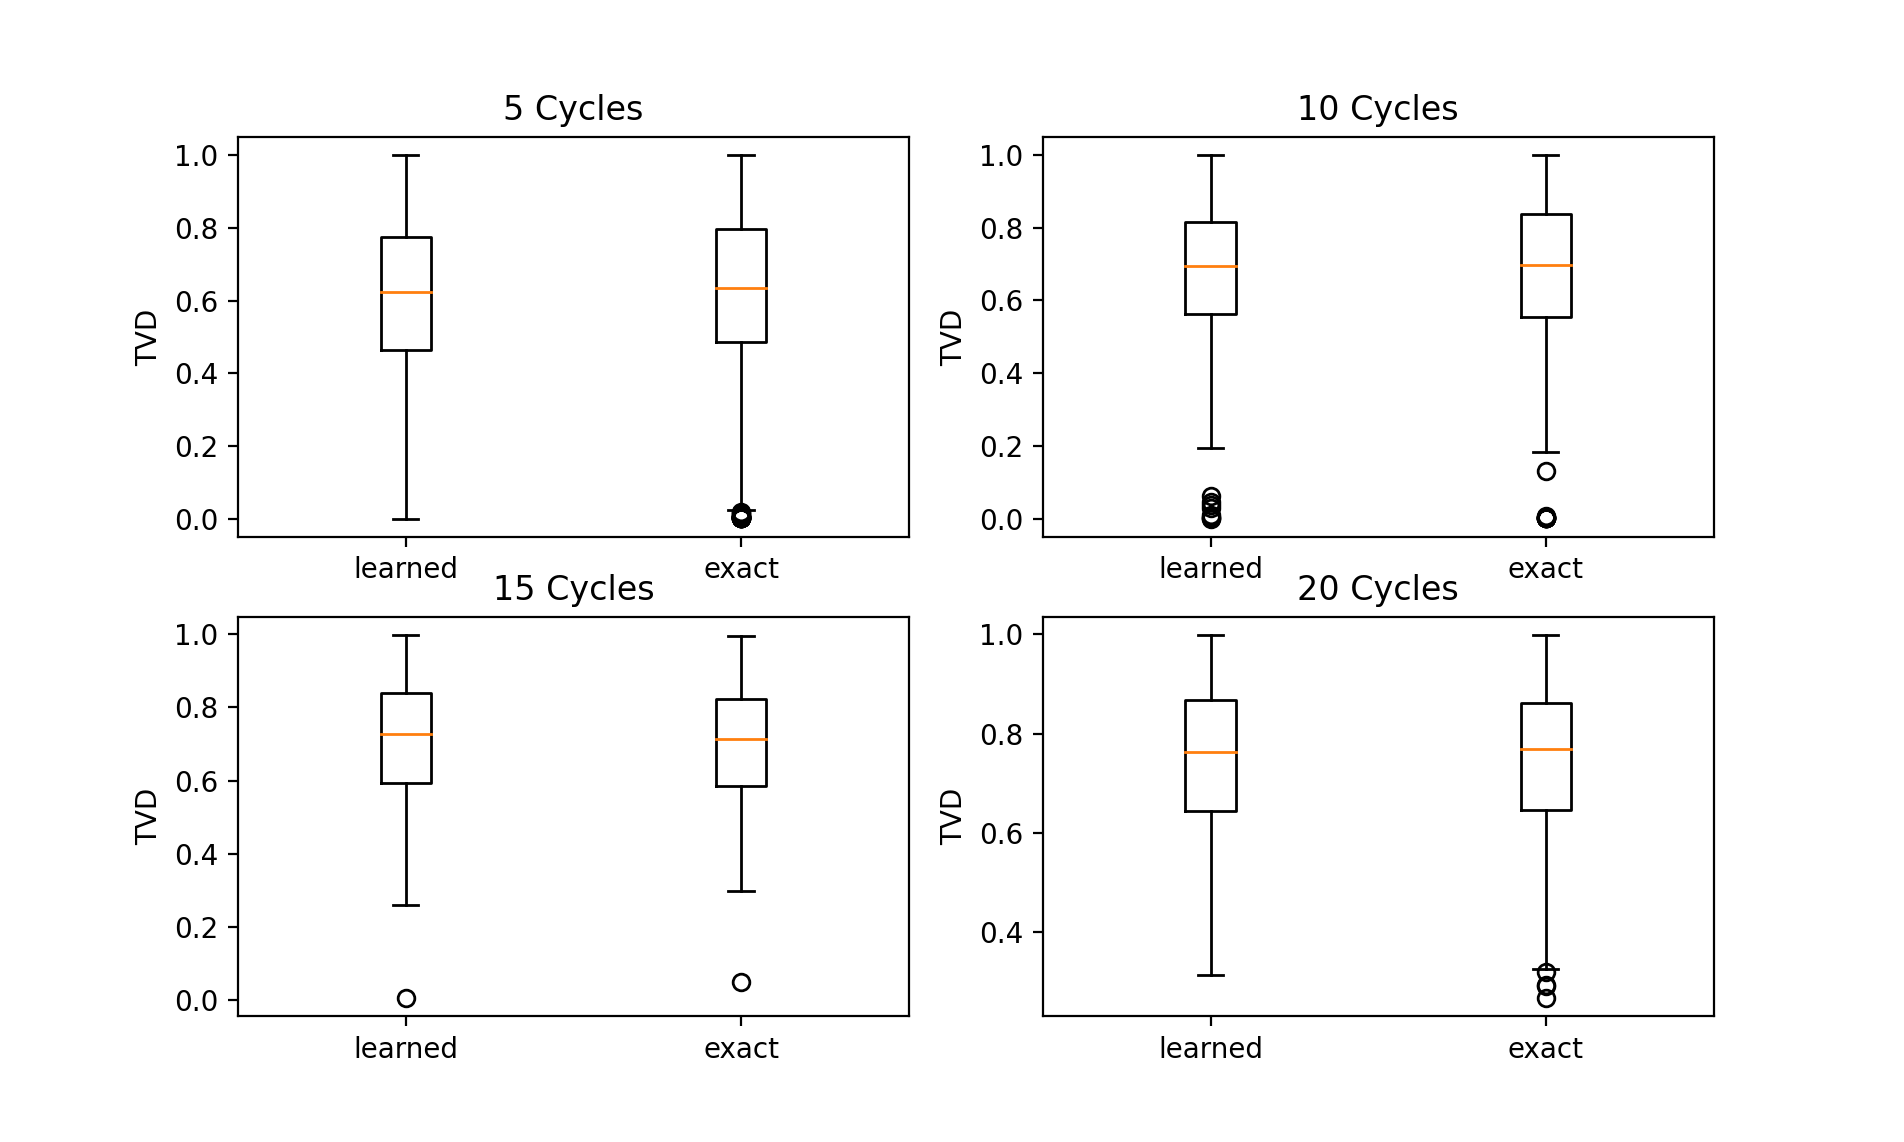
\includegraphics[width=\textwidth]{figures/sr_learned.png}
    \caption[Comparison methods to apply the $CZ$ gate]{TVD of RBMs trained with 
    Stochastic Reconfiguration and random restarts. Once, the $CZ$ gates have been learned and once they have been applied exactly.}
    \label{fig:sr_learned}
  \end{figure}

For 5 cycles, RBMs on which the $CZ$ gate has been applied exactly reach a mean TVD of $0.63$ with a standard deviation of
$\sigma=0.21$ ($0.61$ and $0.21$ when learned). For 10 cycles, the average TVD is $0.68$ and
$\sigma=0.18$ ($0.68$ and $0.17$ when learned). On 15 cycles, with exact $CZ$ gate applications the TVD is at $0.70$ with a standard deviation of $\sigma=0.15$
($0.71$ and $0.16$ when learned). On the biggest circuits with 20 cycles, RBMs with exact $CZ$ gate applications
 reach a mean TVD of $0.75$ with $\sigma=0.15$ ($0.75$ and $0.15$ when the $CZ$ gates were learned).

The $p$ value of the Kruskal-Wallis H test on all circuit instances is $p=0.108$, suggesting that 
that there is no significant difference in learning the $CZ$ gate over adapting the parameters of the 
RBM directly.

The influence of the number of training samples and training iterations on both methods is also analyzed in 
sections X and X.
\fi
\subsection{AdaMax with Random Restarts and CZ Gates Learned}

\begin{figure}[H]
  \centering
  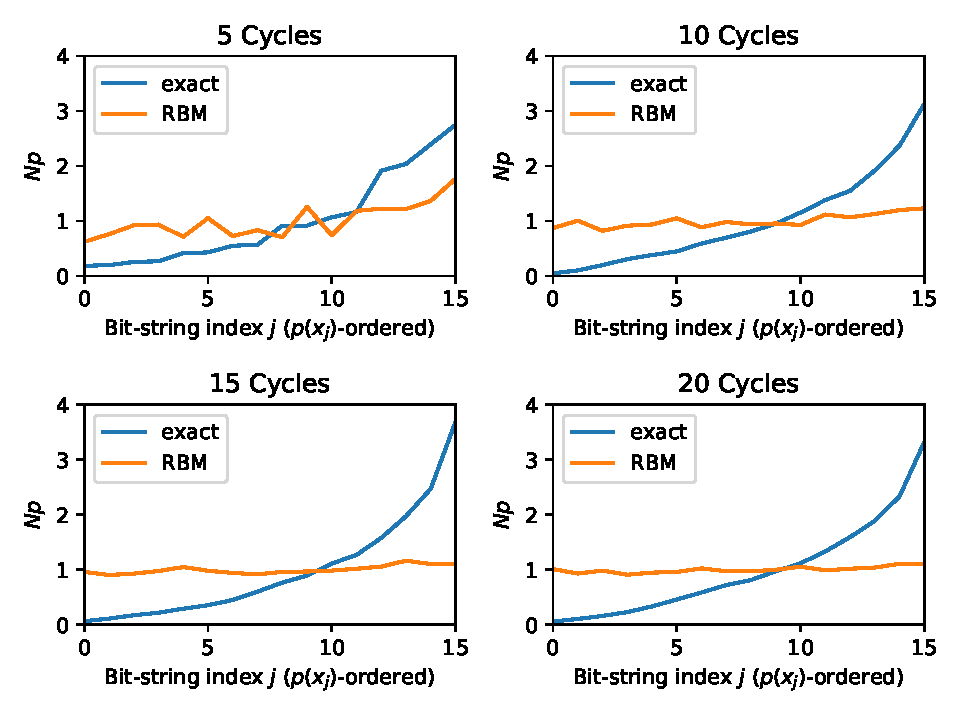
\includegraphics[width=\textwidth]{figures/results/AM-restarts-learned/avgPDF.pdf}
  \caption[Average output probabilities of AdaMax with Restarts Learned]{
    Average output probabilities of AdaMax with Restarts Learned. The true 
    output distribution approaches a Porter-Thomas shape with increasing number of cycles.}
  \label{fig:sr_tvd}
\end{figure}

\begin{figure}[H]
  \centering
  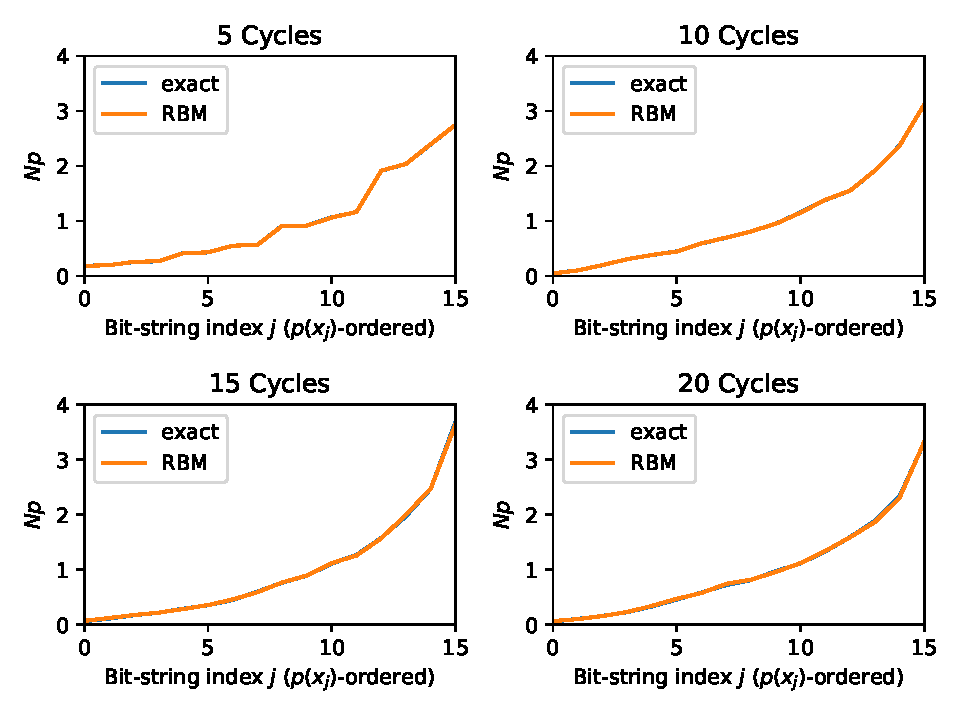
\includegraphics[width=\textwidth]{figures/results/AM-restarts-learned/avgBestPDF.pdf}
  \caption[Averaged best performing output probabilities of AdaMax with Restarts Learned]{
    Average output probabilities of AdaMax with Restarts Learned, only RBMs with lowest
    TVD for each circuit are considered. The true 
    output distribution approaches a Porter-Thomas shape with increasing number of cycles.}
  \label{fig:sr_tvd}
\end{figure}

\begin{figure}[H]
  \centering
  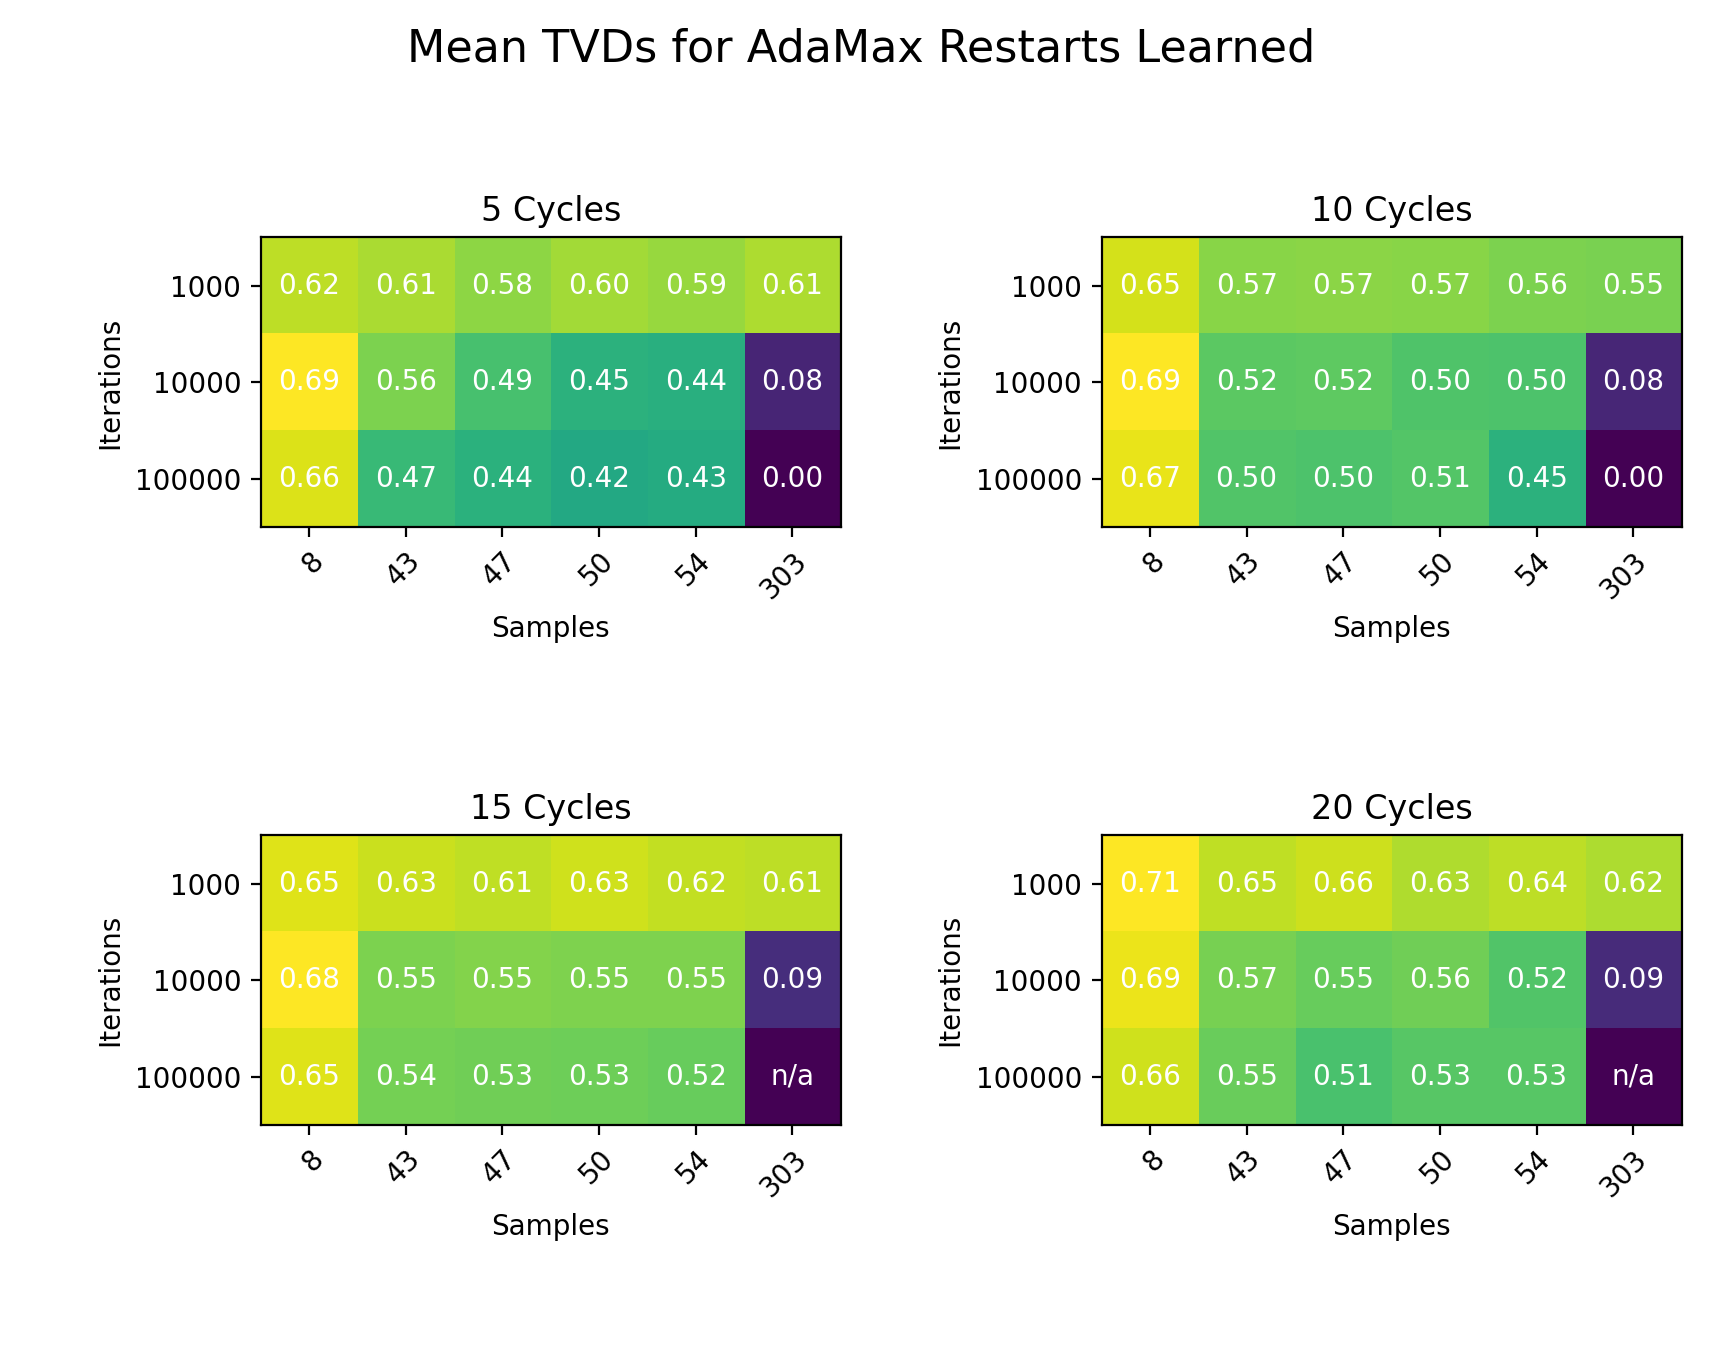
\includegraphics[width=\textwidth]{figures/results/AM-restarts-learned/tvd_heatmap.png}
  \caption[TVD of AdaMax with Restarts Learned]{TVD of Stochastic 
  Reconfiguration with Restarts Learned for the combinations of iterations and samples tested.
  For 100.000 iterations and 303 samples, the experiments did not finish within the time limit.}
  \label{fig:sr_tvd}
\end{figure}

\begin{figure}[H]
  \centering
  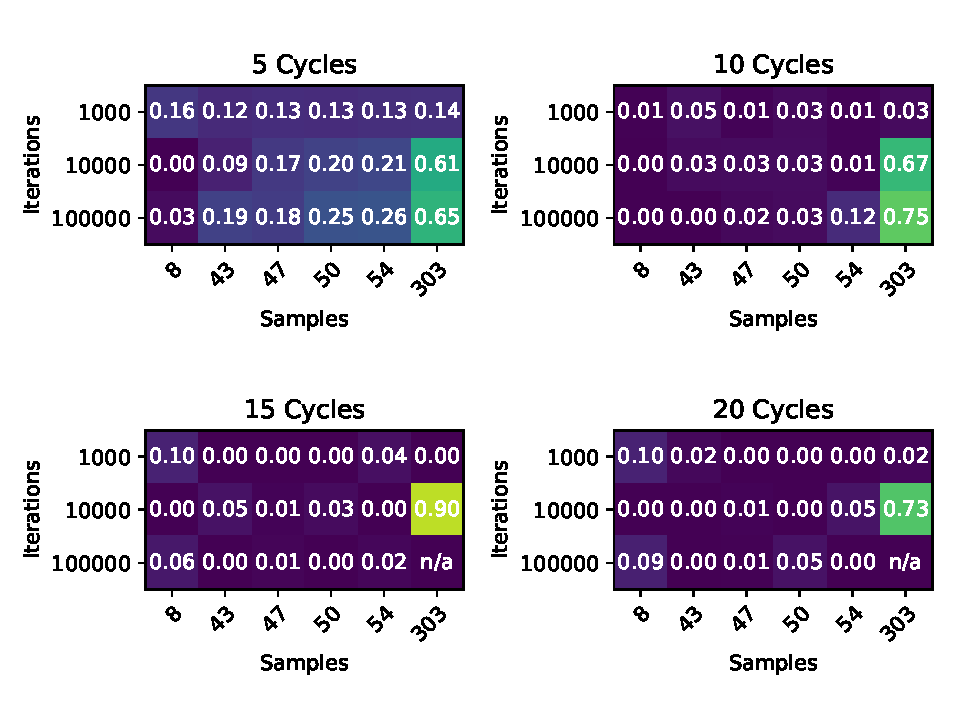
\includegraphics[width=\textwidth]{figures/results/AM-restarts-learned/fxeb_heatmap.pdf}
  \caption[Cross-entropy Fidelity of AdaMax with Restarts Learned]{Cross-entropy Fidelity of Stochastic 
  Reconfiguration with Restarts Learned for the combinations of iterations and samples tested.
  For 100.000 iterations and 303 samples, the experiments did not finish within the time limit.}
  \label{fig:sr_tvd}
\end{figure}


\begin{figure}[H]
  \centering
  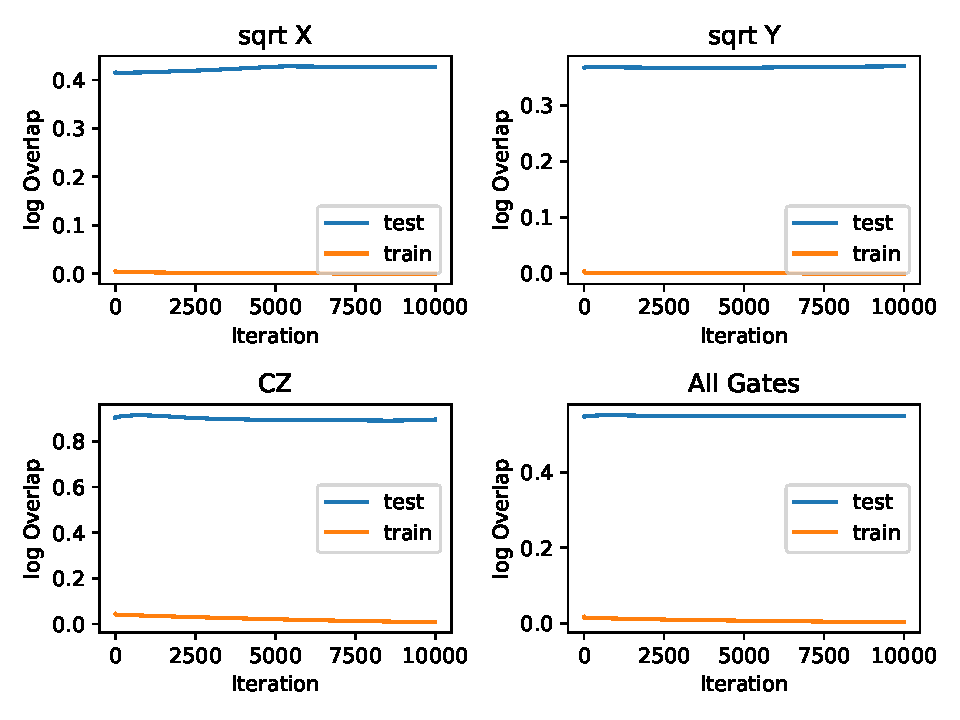
\includegraphics[width=\textwidth]{figures/results/AM-restarts-learned/avgOverlap_8.pdf}
  \caption[Training Overlap of AdaMax with Restarts Learned]{Training 
  Overlap of AdaMax with Restarts Learned for 8 samples.}
  \label{fig:sr_tvd}
\end{figure}

\begin{figure}[H]
  \centering
  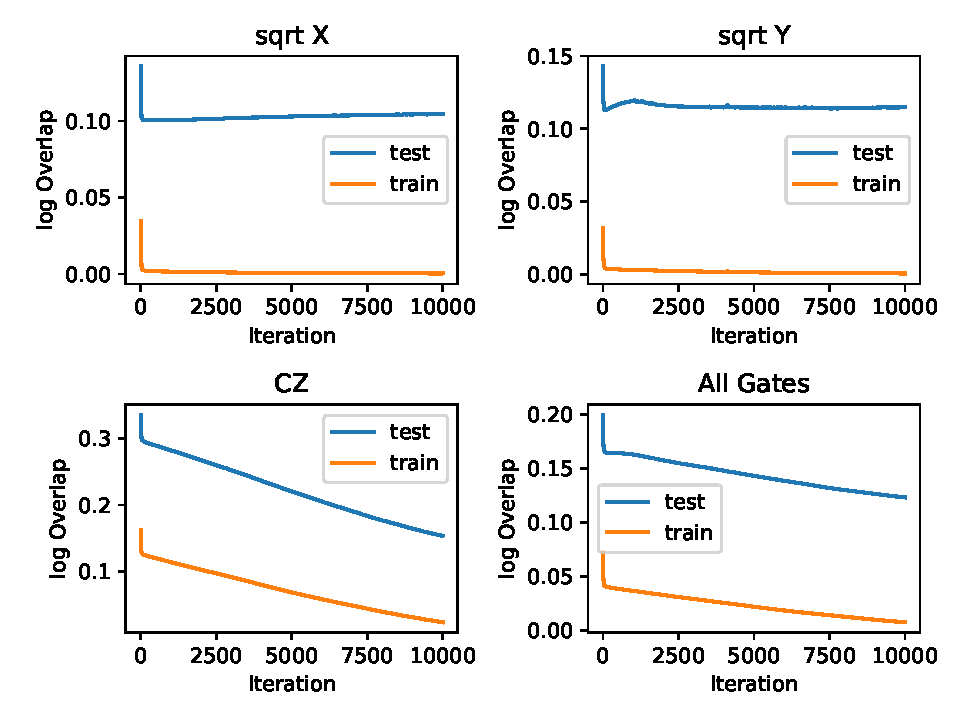
\includegraphics[width=\textwidth]{figures/results/AM-restarts-learned/avgOverlap_47.pdf}
  \caption[Training Overlap of AdaMax with Restarts Learned]{Training 
  Overlap of AdaMax with Restarts Learned for 47 samples.}
  \label{fig:sr_tvd}
\end{figure}

\begin{figure}[H]
  \centering
  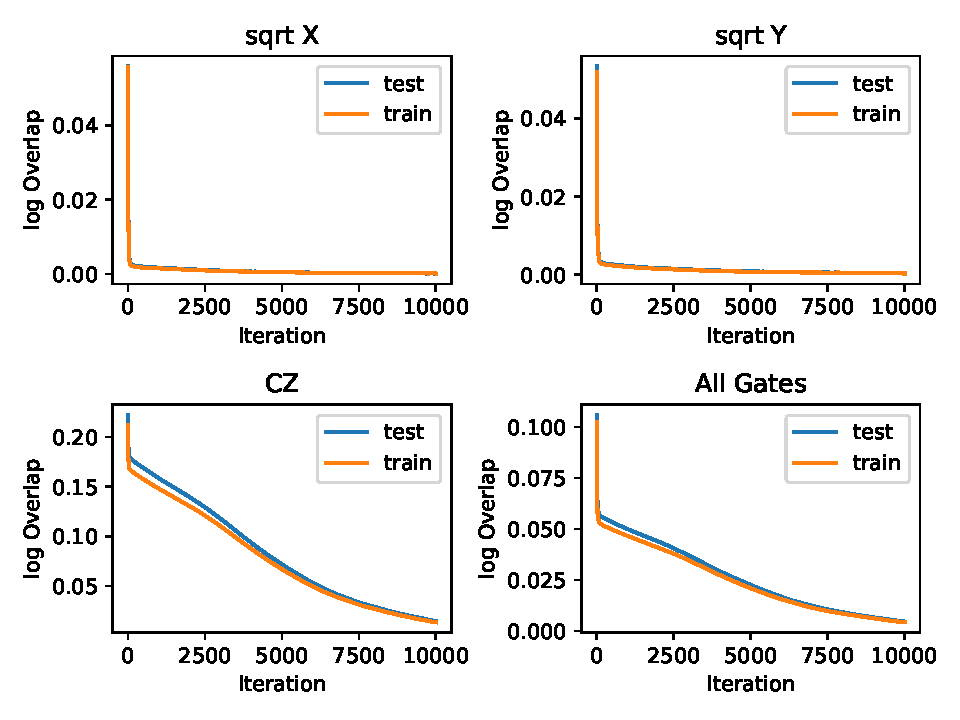
\includegraphics[width=\textwidth]{figures/results/AM-restarts-learned/avgOverlap_303.pdf}
  \caption[Training Overlap of AdaMax with Restarts Learned]{Training 
  Overlap of AdaMax with Restarts Learned for 303 samples.}
  \label{fig:sr_tvd}
\end{figure}
%gate fidelity:  https://en.wikipedia.org/wiki/Fidelity_of_quantum_states

\iffalse
\subsection{Influence of Number of Training Iterations}
Choosing an optimal number of training iterations is a crucial aspect in machine learning.
While too less iterations will lead to poor performance, too many training iterations can lead 
to overfitting \cite{}. The later results in a good performance of the model on the given 
training set but with bad generalization performance on unseen data. 

All described methods have been tested with 1.000, 10.000 and 100.000 training iterations. 
The TVDs by number of training iterations for all four experiments including all numbers 
of training samples and circuit sizes is summarized in figure~\ref{fig:iterations}.

\begin{figure}[H]
    \centering
    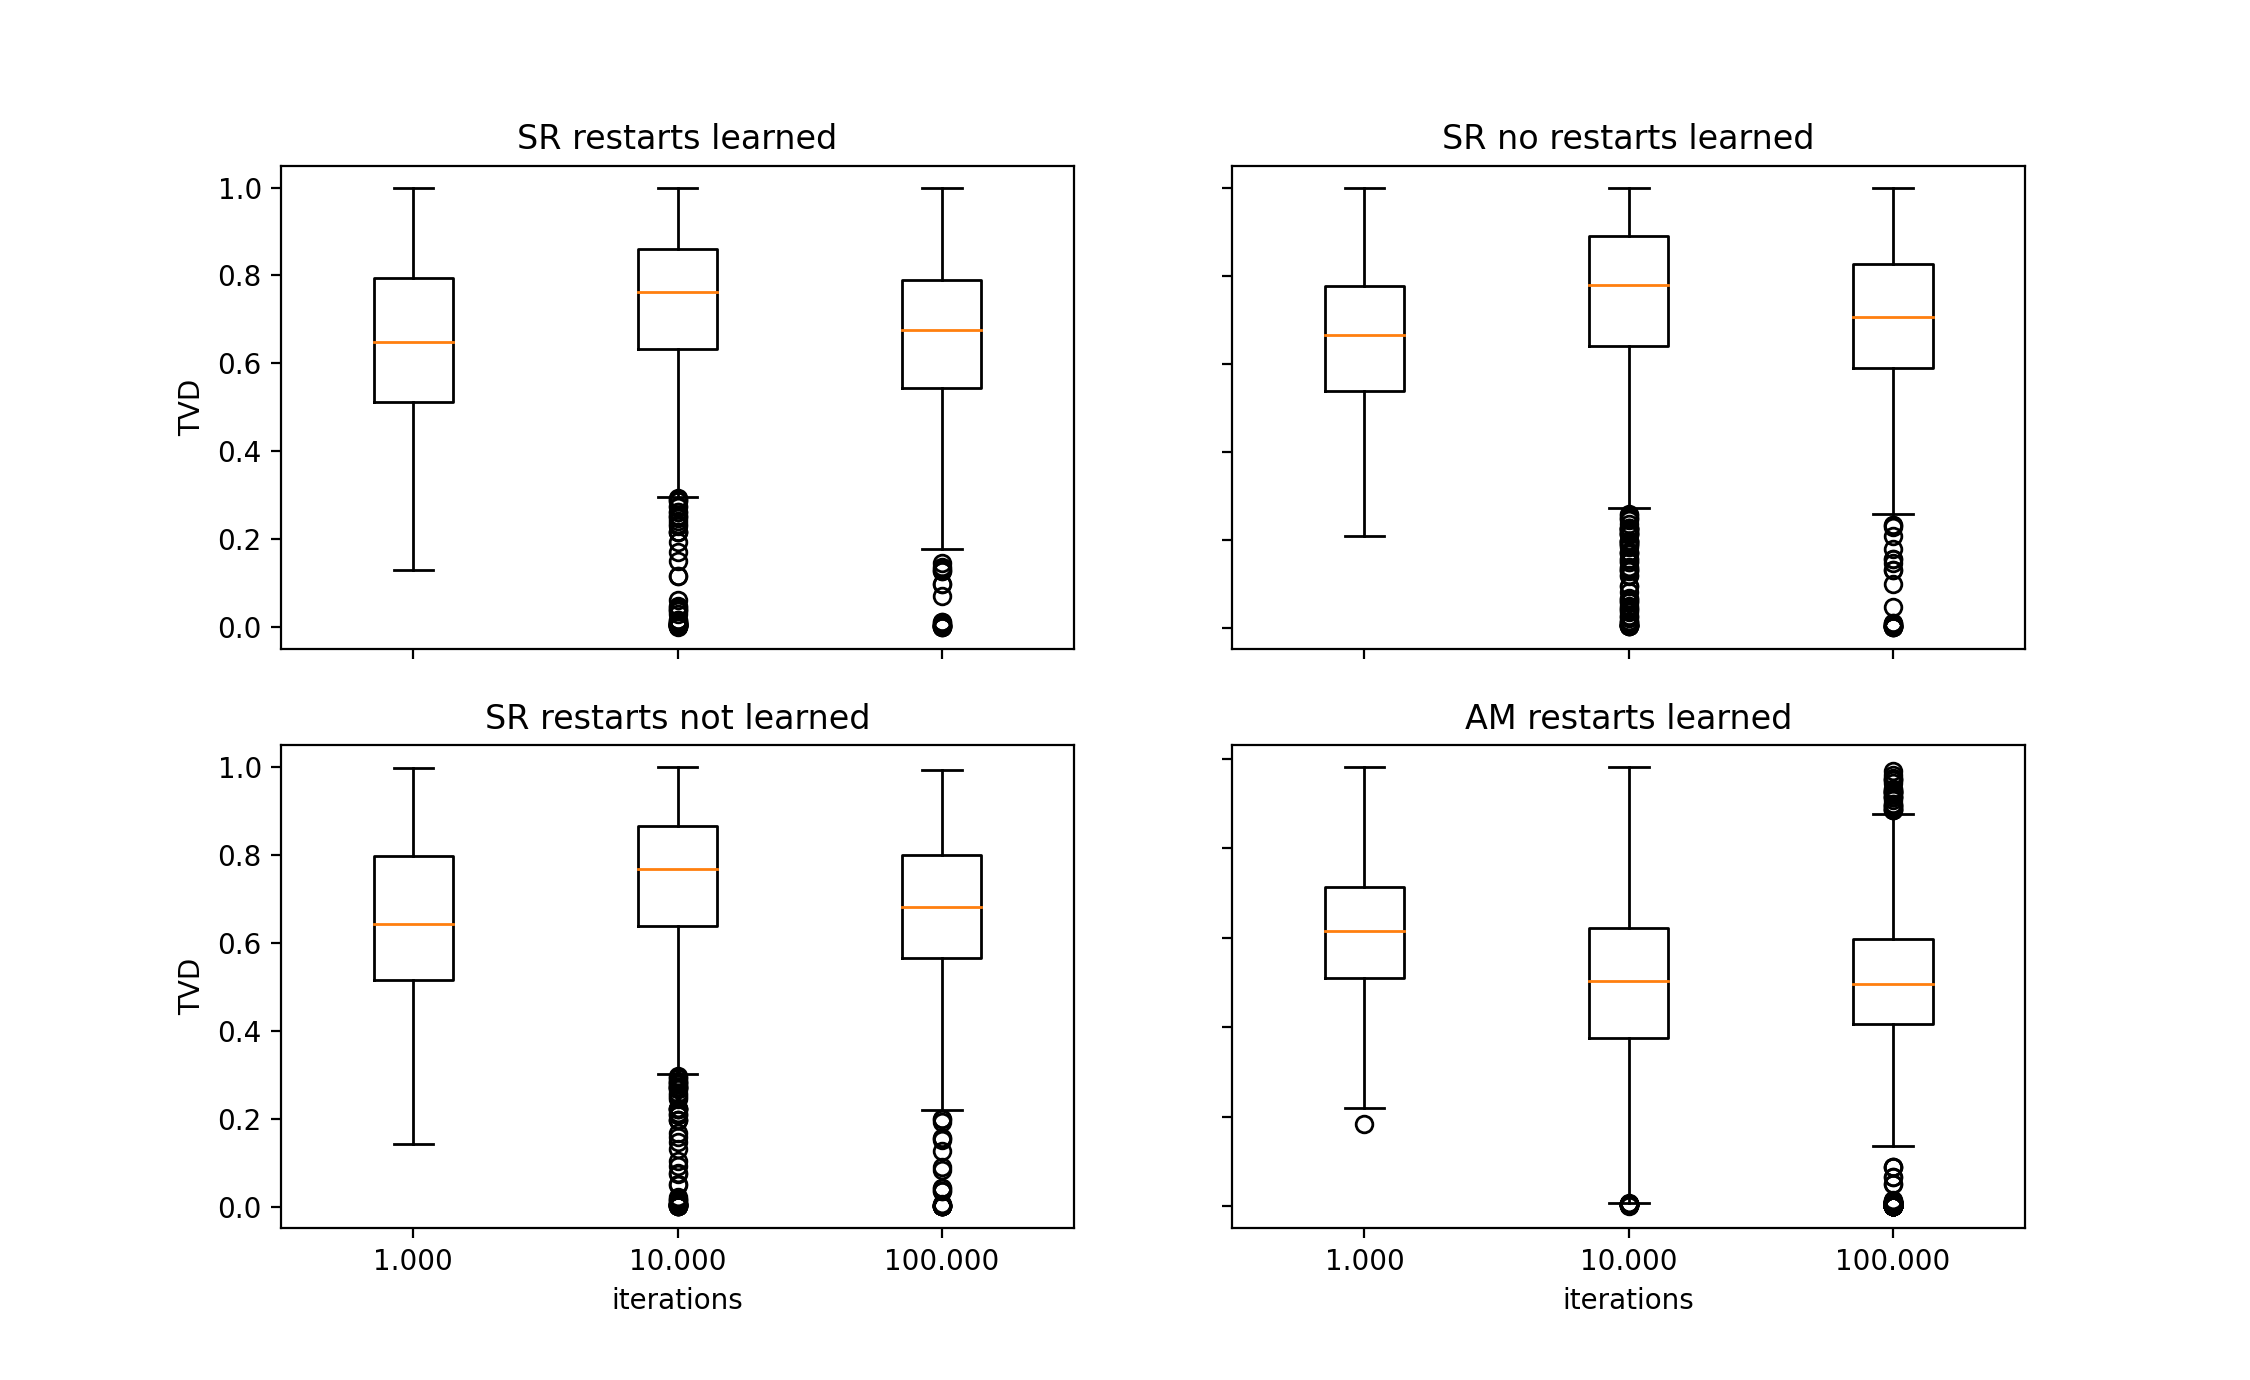
\includegraphics[width=\textwidth]{figures/iterations.png}
    \caption[Influence of Number of Training iterations.]{TVD of RBMs trained with 
    with different number of training iterations. The results include all circuit depths 
    and number of training samples.}
    \label{fig:iterations}
\end{figure}

For SR with restarts and $CZ$ gates learned, the mean TVD is $0.65$ for 1.000, $0.73$ for 10.000 and $0.65$ for 100.000 iterations 
with standard deviations of $\sigma_{1.000}=0.18$, $\sigma_{10.000}=0.18$ and $\sigma_{100.000}=0.19$
each. 

For SR without restarts and the $CZ$ gates learned, the mean TVD is $0.66$ for 1.000, $0.74$ for 10.000 and $0.69$ for 100.000 iterations 
with standard deviations of $\sigma_{1.000}=0.16$, $\sigma_{10.000}=0.19$ and $\sigma_{100.000}=0.19$
each. 

For SR with restarts and exact application of the $CZ$ gate, the mean TVD is $0.65$ for 1.000, $0.74$ for 10.000 and $0.67$ for 100.000 iterations 
with standard deviations of $\sigma_{1.000}=0.18$, $\sigma_{10.000}=0.18$ and $\sigma_{100.000}=0.18$
each. 

For AdaMax, the mean TVD is $0.61$ for 1.000, $0.48$ for 10.000 and $0.48$ for 100.000 iterations 
with standard deviations of $\sigma_{1.000}=0.14$, $\sigma_{10.000}=0.22$ and $\sigma_{100.000}=0.19$
each. 

A look at the averaged log overlap between the RBM's output and the target output distribution
during the training processes shown in figure X reveals more insights on the optimum number of training iterations.

FIGURE HERE

The average number of training iterations at which the test log overlap reaches its minimum is 
X for SR, X for SR without restarts, X for SR with $CZ$ applied exactly and X for AdaMax.


\subsection{Influence of Number of Training Samples}

The number of training samples are an important parameter in the training process of 
Boltzmann machines for the simulation of quantum systems. Exact classical simulation 
techniques have to store all $2^n$ amplitudes of the system's wavefunction. In the worst 
case, the training set for the RBM also has to contain all $2^n$ different states with 
their corresponding amplitudes. In this case, the RBM could be trained to memorize 
the whole wavefunction. 

The number of training samples had been varied from 8, 43, 47, 50, 54, to 303. 
Figure \ref{fig:samples} summarizes the average TVD achieved by the RBMs when 
trained with the given number of training samples averaged over all training iterations and 
circuit sizes.

\begin{figure}[H]
    \centering
    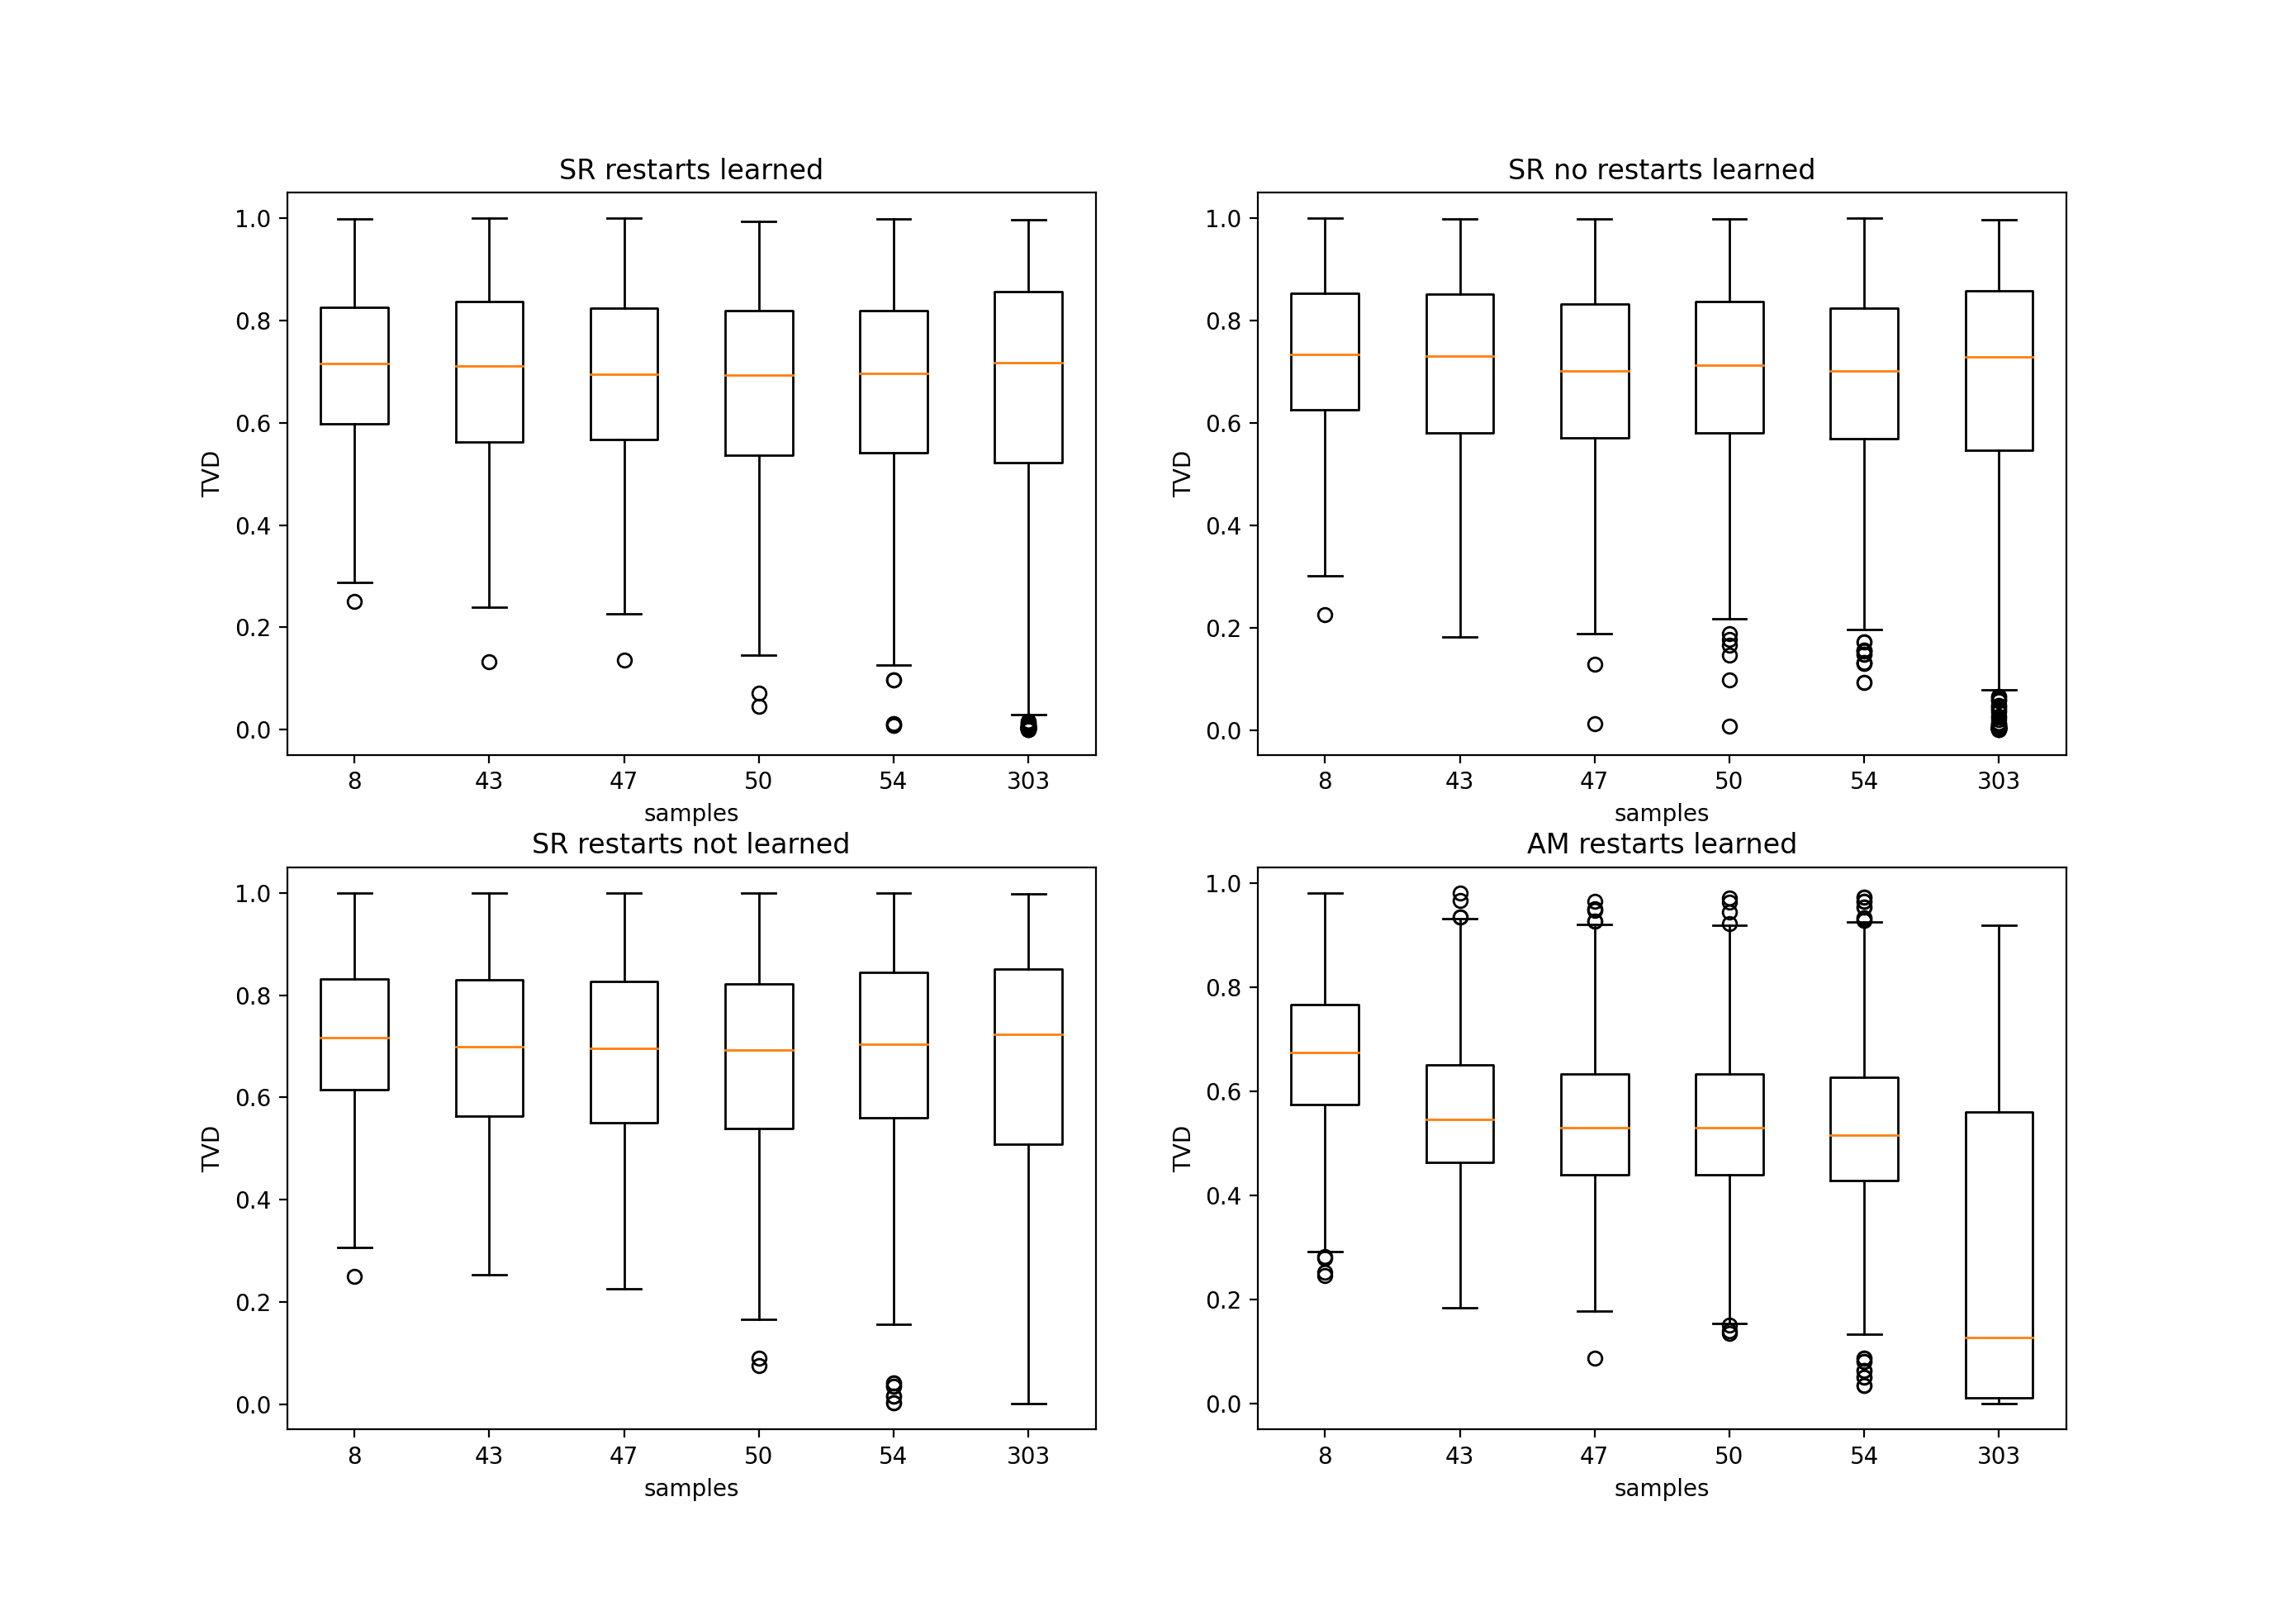
\includegraphics[width=\textwidth]{figures/samples.png}
    \caption[Influence of Number of Training samples.]{TVD of RBMs trained with 
    with different number of training samples. The results include all circuit depths 
    and number of training iterations.}
    \label{fig:samples}
\end{figure}

For AdaMax, the RBMs perform better the more training samples are being used. The RBMs achieve an average 
TVD of 0.67 for 8, 0.56 for 43, 0.54 for 47, 0.54 for 50, 0.53 for 54, and 0.2 for 303 samples. 

For the three different SR methods, this correlation is not as clear as for AdaMax but can still be observed here 
as well. The RBMs achieve an average 
TVD of 0.70/0.73/0.72 for random restarts/without random restarts/exact $CZ$ gate on 8 qubits,
0.70/0.71/0.70 for 43, 0.69/0.69/0.68 for 47, 0.67/0.70/0.68 for 50, 0.67/0.69/0.69 for 54, and 
0.66/0.68/0.66 on 303 samples each.


\subsection{Best Performing RBMs}
For each generated circuit, the training parameters of the best performing RBM have been extracted and 
summarized in table X. It contains the data for 5 and 10 cycles only as some of the experiments timed out 
for many iterations and samples on bigger circuits. Circuits with 15 or 20 cycles have been removed to 
avoid a bias in the data.

table with best trainng params for each experiment.

For AdaMax, the RBM approximates the true output distribution always best with the maximum number of samples (300)
and iterations (100.000). With those settings, the TVD is even 0 for all but one circuit where the TVD is 0.01. The 
RBMs trained with AdaMax and random restarts are thus able to perfectly calculate the output state of random circuit
instances with 4 qubits and 5 and 10 cycles. Also for circuits with 15 and 20 cycles, the best RBMs trained with 
303 samples could approximate the target states very accurate. On those instances, the best performing RBMs trained with 
AdaMax reached an average TVD of X, even with 10.000 training iterations instead of 100.000 but still with 303 training samples.

For the different SR methods, the best RBMs are still able to achieve perfect approximations in some cases. On average, the 
TVD is $0.1$ for SR with restarts and the CZ gates learned, $0.2$ for SR without random restarts and X for SR and the CZ gate not learned.
While most (x out of y) of the best RBMs are still trained with the maximum number of samples, x out of y RBMs reach the best 
approximation with less samples in SR-restarts-learned. For SR-no-restarts-learned its x out of y RBMs with less samples and x out of y 
RBMs for SR-restarts-not-learned that reach the best performance. Also the variation on the number of training iterations is higher
than in the case for AdaMax. 
X out of Y best RBMs are trained with 100.000 iterations in the SR-restarts-learned. For SR-no-restarts-learned it's x out of y 
cases and for SR-restarts-not-learned x out of y. 

So while more training samples and iterations seems to work best for RBMs trained with AdaMax, which could even 
achieve perfect approximations on the given random circuits instances, for SR methods, sometimes less samples and 
iterations led to the best performing RBMs in those cases. These RBMs, however, achieved an average best TVD of 0.2 
compared to 0 for the average best RBMs when trained with AdaMax. These finding underscore the results that 
the number of training iterations does not correlate with RBM performance in the SR cases but in the AdaMax cases.
\fi
